\documentclass[11pt]{article}
\pdfsuppressptexinfo=-1
\usepackage[margin=1in]{geometry}
\usepackage[T1]{fontenc}
\usepackage{booktabs,array,amsmath,amssymb,hyperref,xcolor,graphicx}
\usepackage[numbers]{natbib}
\hypersetup{pdftitle={Do Self-Improving Coding Agents Beat Textbook Baselines? Evidence from a Darwin G\"odel Machine Port and Two Published Systems},pdfauthor={Tejasvi Singh Tomar}}
\newcommand{\nQAcorr}{+6}
\newcommand{\nQAmeas}{+22}
\newcommand{\nQAn}{28}
\newcommand{\nQArho}{0.24}
\newcommand{\nQBcorr}{+6}
\newcommand{\nQBmeas}{+20}
\newcommand{\nQBn}{39}
\newcommand{\nQBrho}{0.94}
\newcommand{\nQCcorr}{+10}
\newcommand{\nQCmeas}{+16}
\newcommand{\nQCn}{26}
\newcommand{\nQCrho}{0.72}
\newcommand{\nQDcorr}{+12}
\newcommand{\nQDmeas}{+20}
\newcommand{\nQDn}{42}
\newcommand{\nQDrho}{0.59}
\newcommand{\nSLoopA}{76}
\newcommand{\nSLoopB}{74}
\newcommand{\nSLoopC}{88}
\newcommand{\nSNohintA}{90}
\newcommand{\nSNohintB}{84}
\newcommand{\nSStrongA}{92}
\newcommand{\nSStrongB}{92}
\newcommand{\nSgainLoopA}{13.5}
\newcommand{\nSgainLoopB}{11.5}
\newcommand{\nSgainLoopC}{25.5}
\newcommand{\nSgainNohintA}{27.5}
\newcommand{\nSgainNohintB}{21.5}
\newcommand{\nSgainStrongA}{7.4}
\newcommand{\nSgainStrongB}{7.4}
\newcommand{\nSrerunLoopA}{72}
\newcommand{\nSrerunLoopB}{70}
\newcommand{\nSrerunStrongA}{89}
\newcommand{\naOneZeroCount}{4}
\newcommand{\nadasArcinfl}{2.3}
\newcommand{\nadasArcrho}{0.60}
\newcommand{\nadasDropinfl}{2.8}
\newcommand{\nadasDroprho}{0.89}
\newcommand{\nadasGpqabaseShift}{-2.7}
\newcommand{\nadasGpqabestBaseLoss}{-1.4}
\newcommand{\nadasGpqagainOverBestBase}{+0.9}
\newcommand{\nadasGpqainfl}{6.5}
\newcommand{\nadasGpqarho}{0.08}
\newcommand{\nadasMgsminfl}{1.3}
\newcommand{\nadasMgsmrho}{0.86}
\newcommand{\nadasMmlubaseShift}{+4.5}
\newcommand{\nadasMmlubestBaseLoss}{9.9}
\newcommand{\nadasMmlugainOverBestBase}{+5.6}
\newcommand{\nadasMmluinfl}{9.8}
\newcommand{\nadasMmlurho}{0.25}
\newcommand{\natkDgmEight}{73.4}
\newcommand{\natkDgmEightusd}{10.4}
\newcommand{\natkDgmOne}{65.6}
\newcommand{\natkDgmOneusd}{3.9}
\newcommand{\natkDgmSix}{72.9}
\newcommand{\natkDgmSixusd}{8.8}
\newcommand{\natkDgmThree}{71.2}
\newcommand{\natkDgmThreeusd}{6.1}
\newcommand{\natkDgmTwelve}{73.9}
\newcommand{\natkDgmTwelveusd}{13.6}
\newcommand{\natkDgmTwo}{69.7}
\newcommand{\natkDgmTwousd}{5.1}
\newcommand{\natkDgmkmax}{12}
\newcommand{\natkStrongEight}{89.3}
\newcommand{\natkStrongEightusd}{22.6}
\newcommand{\natkStrongOne}{86.0}
\newcommand{\natkStrongOneusd}{8.8}
\newcommand{\natkStrongSix}{88.7}
\newcommand{\natkStrongSixusd}{19.3}
\newcommand{\natkStrongThree}{87.7}
\newcommand{\natkStrongThreeusd}{13.5}
\newcommand{\natkStrongTwo}{87.2}
\newcommand{\natkStrongTwousd}{11.3}
\newcommand{\natkStrongkmax}{8}
\newcommand{\nbgenLoopA}{3}
\newcommand{\nbgenLoopB}{4}
\newcommand{\nbgenLoopC}{25}
\newcommand{\nbgenNohintA}{40}
\newcommand{\nbgenNohintB}{25}
\newcommand{\nbgenStrongA}{11}
\newcommand{\nbgenStrongB}{29}
\newcommand{\ncapFone}{85.6}
\newcommand{\ncapGain}{+20.0}
\newcommand{\ncapGainhi}{+26.2}
\newcommand{\ncapGainlo}{+14.1}
\newcommand{\ncapUsd}{7.0}
\newcommand{\nconLfiveMinusLfour}{+4.3}
\newcommand{\nconLfourMinusLtwo}{+6.9}
\newcommand{\nconLone}{+2.3}
\newcommand{\nconLtwoMinusLone}{+1.1}
\newcommand{\ncostRatioRange}{2 to 13}
\newcommand{\nctwoEmptyFail}{0}
\newcommand{\nctwoEmptyOK}{14}
\newcommand{\nctwoStochFail}{9}
\newcommand{\nctwoStochOK}{0}
\newcommand{\nctwoTaskOK}{1}
\newcommand{\nfoneLoopA}{75.0}
\newcommand{\nfoneLoopB}{76.7}
\newcommand{\nfoneLoopC}{88.8}
\newcommand{\nfoneNohintA}{87.1}
\newcommand{\nfoneNohintB}{87.9}
\newcommand{\nfoneStrongA}{87.9}
\newcommand{\nfoneStrongB}{87.9}
\newcommand{\ngainLoopA}{9.4}
\newcommand{\ngainLoopAhi}{+14.2}
\newcommand{\ngainLoopAlo}{+5.3}
\newcommand{\ngainLoopB}{11.1}
\newcommand{\ngainLoopBhi}{+15.9}
\newcommand{\ngainLoopBlo}{+6.9}
\newcommand{\ngainLoopC}{23.2}
\newcommand{\ngainLoopChi}{+30.2}
\newcommand{\ngainLoopClo}{+16.8}
\newcommand{\ngainNohintA}{21.5}
\newcommand{\ngainNohintAhi}{+28.8}
\newcommand{\ngainNohintAlo}{+14.3}
\newcommand{\ngainNohintB}{22.3}
\newcommand{\ngainNohintBhi}{+29.7}
\newcommand{\ngainNohintBlo}{+15.5}
\newcommand{\ngainStrongA}{1.8}
\newcommand{\ngainStrongAhi}{+4.7}
\newcommand{\ngainStrongAlo}{-0.9}
\newcommand{\ngainStrongB}{1.8}
\newcommand{\ngainStrongBhi}{+4.2}
\newcommand{\ngainStrongBlo}{+0.1}
\newcommand{\ngainallLoopA}{7.0}
\newcommand{\ngainallLoopAhi}{+10.3}
\newcommand{\ngainallLoopAlo}{+4.0}
\newcommand{\ngainallLoopB}{9.2}
\newcommand{\ngainallLoopBhi}{+12.9}
\newcommand{\ngainallLoopBlo}{+5.6}
\newcommand{\ngainallStrongA}{2.4}
\newcommand{\ngainallStrongAhi}{+4.7}
\newcommand{\ngainallStrongAlo}{+0.0}
\newcommand{\ngenLoopA}{40}
\newcommand{\ngenLoopB}{40}
\newcommand{\ngenLoopC}{40}
\newcommand{\ngenNohintA}{40}
\newcommand{\ngenNohintB}{40}
\newcommand{\ngenStrongA}{40}
\newcommand{\ngenStrongB}{40}
\newcommand{\nhFiveDiff}{Haiku 4.5 -7.7 [-18.7, +2.7]; Sonnet 4.6 -11.1 [-20.3, -1.7]}
\newcommand{\nhFourCI}{+2.4 [90\% CI +0.5, +4.3]}
\newcommand{\nhTwoInfl}{6.5 [-1.5, +15.4]; 2.3 [-5.2, +10.8]; 2.3 [-10.1, +15.3]}
\newcommand{\nladCone}{+2.3}
\newcommand{\nladConeatt}{24}
\newcommand{\nladConebest}{+3.4}
\newcommand{\nladConebestS}{68}
\newcommand{\nladConefail}{2}
\newcommand{\nladConehi}{+4.2}
\newcommand{\nladConeitt}{+2.1}
\newcommand{\nladConelo}{+0.4}
\newcommand{\nladConen}{22}
\newcommand{\nladCthree}{+1.6}
\newcommand{\nladCthreeatt}{24}
\newcommand{\nladCthreebest}{+0.8}
\newcommand{\nladCthreebestS}{68}
\newcommand{\nladCthreefail}{0}
\newcommand{\nladCthreehi}{+4.1}
\newcommand{\nladCthreeitt}{+1.6}
\newcommand{\nladCthreelo}{-0.7}
\newcommand{\nladCthreen}{24}
\newcommand{\nladCtwo}{+6.3}
\newcommand{\nladCtwoatt}{24}
\newcommand{\nladCtwobest}{+10.3}
\newcommand{\nladCtwobestS}{72}
\newcommand{\nladCtwofail}{9}
\newcommand{\nladCtwohi}{+9.5}
\newcommand{\nladCtwoitt}{+3.9}
\newcommand{\nladCtwolo}{+3.4}
\newcommand{\nladCtwon}{15}
\newcommand{\nladDone}{+2.9}
\newcommand{\nladDoneatt}{10}
\newcommand{\nladDonebest}{+4.2}
\newcommand{\nladDonebestS}{68}
\newcommand{\nladDonefail}{8}
\newcommand{\nladDonehi}{+6.6}
\newcommand{\nladDoneitt}{+0.6}
\newcommand{\nladDonelo}{-1.1}
\newcommand{\nladDonen}{2}
\newcommand{\nladDtwo}{+5.7}
\newcommand{\nladDtwoatt}{10}
\newcommand{\nladDtwobest}{+7.7}
\newcommand{\nladDtwobestS}{68}
\newcommand{\nladDtwofail}{6}
\newcommand{\nladDtwohi}{+9.8}
\newcommand{\nladDtwoitt}{+2.3}
\newcommand{\nladDtwolo}{+1.9}
\newcommand{\nladDtwon}{4}
\newcommand{\nladSCone}{+1.2}
\newcommand{\nladSConeatt}{16}
\newcommand{\nladSConebest}{+1.8}
\newcommand{\nladSConebestS}{88}
\newcommand{\nladSConefail}{0}
\newcommand{\nladSConehi}{+3.7}
\newcommand{\nladSConeitt}{+1.2}
\newcommand{\nladSConelo}{-1.0}
\newcommand{\nladSConen}{16}
\newcommand{\nladSCtwo}{-4.1}
\newcommand{\nladSCtwoatt}{16}
\newcommand{\nladSCtwobest}{+1.0}
\newcommand{\nladSCtwobestS}{86}
\newcommand{\nladSCtwofail}{0}
\newcommand{\nladSCtwohi}{+0.1}
\newcommand{\nladSCtwoitt}{-4.1}
\newcommand{\nladSCtwolo}{-9.5}
\newcommand{\nladSCtwon}{16}
\newcommand{\nlinCempty}{4}
\newcommand{\nlinCn}{6}
\newcommand{\nnohintPairText}{+21.5 and +22.3 points}
\newcommand{\norcDgmEight}{74.1}
\newcommand{\norcDgmOne}{65.6}
\newcommand{\norcDgmSix}{73.5}
\newcommand{\norcDgmThree}{71.6}
\newcommand{\norcDgmTwelve}{75.0}
\newcommand{\norcDgmTwo}{70.1}
\newcommand{\norcStrongEight}{90.5}
\newcommand{\norcStrongOne}{86.0}
\newcommand{\norcStrongSix}{89.8}
\newcommand{\norcStrongThree}{88.5}
\newcommand{\norcStrongTwo}{87.7}
\newcommand{\npilotInF}{19}
\newcommand{\nplaceboBestA}{68}
\newcommand{\nplaceboBestB}{70}
\newcommand{\nplaceboBestC}{68}
\newcommand{\nplaceboGainRange}{5.5 to 7.5}
\newcommand{\nplaceboNA}{81}
\newcommand{\nplaceboNB}{81}
\newcommand{\nplaceboNC}{81}
\newcommand{\nplaceboNtext}{81 copies each}
\newcommand{\nplaceboPredA}{69.3}
\newcommand{\nplaceboPredB}{69.3}
\newcommand{\nplaceboPredC}{69.3}
\newcommand{\nplaceboPredText}{69.3\% for each loop}
\newcommand{\nquirkStrongCorrText}{+6 points each}
\newcommand{\nquirkStrongMeasText}{+22 and +20 points}
\newcommand{\nretroPolyHeld}{14}
\newcommand{\nretroPolySel}{24}
\newcommand{\nretroSweOther}{50.4}
\newcommand{\nretroSweSel}{50.0}
\newcommand{\nseedDgmFall}{65.8}
\newcommand{\nseedDgmFone}{65.6}
\newcommand{\nseedDgmSmax}{70}
\newcommand{\nseedDgmSmean}{62.5}
\newcommand{\nseedDgmSn}{254}
\newcommand{\nseedDgmSsd}{2.8}
\newcommand{\nseedEmptyOfFail}{80}
\newcommand{\nseedEmptyShare}{28}
\newcommand{\nseedStrongFall}{86.0}
\newcommand{\nseedStrongFone}{86.1}
\newcommand{\nseedStrongSmax}{90}
\newcommand{\nseedStrongSmean}{84.6}
\newcommand{\nseedStrongSn}{85}
\newcommand{\nseedStrongSsd}{2.4}
\newcommand{\nstrongMinusDgmAll}{20.2}
\newcommand{\nstrongMinusDgmNP}{18.9}
\newcommand{\nstrongPlaceboBest}{90}
\newcommand{\nstrongPlaceboGen}{40}
\newcommand{\nstrongPlaceboN}{81}
\newcommand{\nstrongPlaceboPred}{90.4}
\newcommand{\nswapLinesText}{broken edits changed 247--448 lines, working ones 70--253}
\newcommand{\nswapText}{The seed agent returned no edit for 5 of the 12 diagnoses, and 7 working agents remained (mean selection score 66.0\%; mean fresh gain +4.6 points over 7 with fresh results). Loop 3's best agent returned an edit for every diagnosis; 5 of its edits left an agent that wrote no solution, and 7 working agents remained (mean selection score 66.9\%; mean fresh gain +6.0 points over 7 with fresh results).}
\newcommand{\ntrGemcapSeed}{0}
\newcommand{\ntrGemcapThree}{0}
\newcommand{\ntrGemone}{+32.8}
\newcommand{\ntrGemonehi}{+41.4}
\newcommand{\ntrGemonelo}{+24.1}
\newcommand{\ntrGemseed}{12.1}
\newcommand{\ntrGemstrong}{30.2}
\newcommand{\ntrGemthree}{+38.8}
\newcommand{\ntrGemthreehi}{+47.4}
\newcommand{\ntrGemthreelo}{+30.2}
\newcommand{\ntrHfourcapSeed}{0}
\newcommand{\ntrHfourcapThree}{77}
\newcommand{\ntrHfourone}{+1.7}
\newcommand{\ntrHfouronehi}{+8.6}
\newcommand{\ntrHfouronelo}{-5.2}
\newcommand{\ntrHfourseed}{25.0}
\newcommand{\ntrHfourstrong}{47.4}
\newcommand{\ntrHfourthree}{+15.5}
\newcommand{\ntrHfourthreehi}{+22.4}
\newcommand{\ntrHfourthreelo}{+7.8}
\newcommand{\ntrOsscapSeed}{0}
\newcommand{\ntrOsscapThree}{0}
\newcommand{\ntrOssone}{-5.2}
\newcommand{\ntrOssonehi}{+3.4}
\newcommand{\ntrOssonelo}{-13.8}
\newcommand{\ntrOssseed}{40.5}
\newcommand{\ntrOssstrong}{25.9}
\newcommand{\ntrOssthree}{+22.4}
\newcommand{\ntrOssthreehi}{+31.9}
\newcommand{\ntrOssthreelo}{+12.9}
\newcommand{\ntrSfivecapSeed}{0}
\newcommand{\ntrSfivecapThree}{1}
\newcommand{\ntrSfiveone}{+2.6}
\newcommand{\ntrSfiveonehi}{+6.0}
\newcommand{\ntrSfiveonelo}{+0.0}
\newcommand{\ntrSfiveseed}{87.9}
\newcommand{\ntrSfivestrong}{90.5}
\newcommand{\ntrSfivethree}{+3.4}
\newcommand{\ntrSfivethreehi}{+6.9}
\newcommand{\ntrSfivethreelo}{+0.9}
\newcommand{\ntrSfourcapSeed}{9}
\newcommand{\ntrSfourcapThree}{52}
\newcommand{\ntrSfourone}{+6.0}
\newcommand{\ntrSfouronehi}{+13.8}
\newcommand{\ntrSfouronelo}{-2.6}
\newcommand{\ntrSfourseed}{58.6}
\newcommand{\ntrSfourstrong}{76.7}
\newcommand{\ntrSfourthree}{+12.1}
\newcommand{\ntrSfourthreehi}{+19.8}
\newcommand{\ntrSfourthreelo}{+5.2}
\newcommand{\nusdLoopA}{11.7}
\newcommand{\nusdLoopB}{11.3}
\newcommand{\nusdLoopC}{18.7}
\newcommand{\nusdNohintA}{17.2}
\newcommand{\nusdNohintB}{19.1}
\newcommand{\nusdStrongA}{12.1}
\newcommand{\nusdStrongB}{15.4}
\newcommand{\nverdictFive}{not established}
\newcommand{\nverdictFour}{not established}
\newcommand{\nverdictOne}{supported}
\newcommand{\nverdictThree}{not supported}
\newcommand{\nverdictTwo}{not supported}
\newcommand{\nvskLoopA}{+1.3}
\newcommand{\nvskLoopAhi}{+5.8}
\newcommand{\nvskLoopAk}{10}
\newcommand{\nvskLoopAlo}{-2.7}
\newcommand{\nvskLoopB}{+3.1}
\newcommand{\nvskLoopBhi}{+6.3}
\newcommand{\nvskLoopBk}{10}
\newcommand{\nvskLoopBlo}{+0.5}
\newcommand{\nvskLoopC}{+14.9}
\newcommand{\nvskLoopChi}{+21.6}
\newcommand{\nvskLoopCk}{12}
\newcommand{\nvskLoopClo}{+8.8}
\newcommand{\nvskNohintA}{+13.1}
\newcommand{\nvskNohintAhi}{+20.0}
\newcommand{\nvskNohintAk}{12}
\newcommand{\nvskNohintAlo}{+6.4}
\newcommand{\nvskNohintB}{+14.0}
\newcommand{\nvskNohintBhi}{+20.8}
\newcommand{\nvskNohintBk}{12}
\newcommand{\nvskNohintBlo}{+7.5}
\newcommand{\nvskStrongA}{+0.2}
\newcommand{\nvskStrongAhi}{+2.4}
\newcommand{\nvskStrongAk}{3}
\newcommand{\nvskStrongAlo}{-2.2}
\newcommand{\nvskStrongB}{-0.2}
\newcommand{\nvskStrongBhi}{+1.5}
\newcommand{\nvskStrongBk}{4}
\newcommand{\nvskStrongBlo}{-2.2}

\newcommand{\vHeightOpusbest}{-4.3}
\newcommand{\vHeightOpusbestAbs}{4.3}
\newcommand{\vHeightOpusbestAbshi}{7.8}
\newcommand{\vHeightOpusbestAbslo}{1.3}
\newcommand{\vHeightOpusbestVerdict}{not supported}
\newcommand{\vHeightOpusbesthi}{-1.3}
\newcommand{\vHeightOpusbestlo}{-7.8}
\newcommand{\vHeightOpusmean}{+2.6}
\newcommand{\vHeightOpusmeanVerdict}{supported}
\newcommand{\vHeightOpusmeanhi}{+4.6}
\newcommand{\vHeightOpusmeanlo}{+0.6}
\newcommand{\vHeightSonnetbest}{-4.7}
\newcommand{\vHeightSonnetbestAbs}{4.7}
\newcommand{\vHeightSonnetbestAbshi}{8.6}
\newcommand{\vHeightSonnetbestAbslo}{1.3}
\newcommand{\vHeightSonnetbestVerdict}{not supported}
\newcommand{\vHeightSonnetbesthi}{-1.3}
\newcommand{\vHeightSonnetbestlo}{-8.6}
\newcommand{\vHeightSonnetmean}{+0.3}
\newcommand{\vHeightSonnetmeanVerdict}{supported}
\newcommand{\vHeightSonnetmeanhi}{+1.8}
\newcommand{\vHeightSonnetmeanlo}{-1.3}
\newcommand{\vHsixEBLP}{-2.4}
\newcommand{\vHsixEBLPhi}{+0.2}
\newcommand{\vHsixEBLPlo}{-5.0}
\newcommand{\vHsixFtwo}{-4.7}
\newcommand{\vHsixFtwoAbs}{4.7}
\newcommand{\vHsixFtwoAbshi}{9.5}
\newcommand{\vHsixFtwoAbslo}{0.4}
\newcommand{\vHsixFtwohi}{-0.4}
\newcommand{\vHsixFtwolo}{-9.5}
\newcommand{\vHsixL}{-1.7}
\newcommand{\vHsixLAbs}{1.7}
\newcommand{\vHsixLAbshi}{3.2}
\newcommand{\vHsixLAbslo}{0.4}
\newcommand{\vHsixLhi}{-0.4}
\newcommand{\vHsixLlo}{-3.2}
\newcommand{\vHsixVerdict}{not supported}
\newcommand{\vHsixWinner}{EBLP}
\newcommand{\vLVsCapFin}{+1.3}
\newcommand{\vLVsCapFinhi}{+3.4}
\newcommand{\vLVsCapFinlo}{-0.9}
\newcommand{\vLoneAcc}{86.9}
\newcommand{\vLoneMinusLoop}{-1.7}
\newcommand{\vLoneMinusLoophi}{-0.4}
\newcommand{\vLoneMinusLooplo}{-3.2}
\newcommand{\vLoneUsd}{8.7}
\newcommand{\vLthreeAcc}{88.6}
\newcommand{\vLthreeUsd}{19.3}
\newcommand{\vLtwoAcc}{88.4}
\newcommand{\vLtwoCostShare}{59}
\newcommand{\vLtwoMinusLoop}{-0.2}
\newcommand{\vLtwoMinusLoophi}{+0.6}
\newcommand{\vLtwoMinusLooplo}{-1.3}
\newcommand{\vLtwoUsd}{11.4}
\newcommand{\vadasDrop}{-6.1}
\newcommand{\vadasDropN}{10}
\newcommand{\vadasDroparch}{+6.3}
\newcommand{\vadasDrophi}{-4.2}
\newcommand{\vadasDroplo}{-8.1}
\newcommand{\vadasGpqa}{+3.3}
\newcommand{\vadasGpqaN}{16}
\newcommand{\vadasGpqaarch}{+1.8}
\newcommand{\vadasGpqahi}{+5.4}
\newcommand{\vadasGpqalo}{+1.4}
\newcommand{\vadasMgsm}{-2.0}
\newcommand{\vadasMgsmN}{5}
\newcommand{\vadasMgsmarch}{+25.2}
\newcommand{\vadasMgsmhi}{-0.8}
\newcommand{\vadasMgsmlo}{-3.2}
\newcommand{\vadasMmlu}{-0.1}
\newcommand{\vadasMmluN}{4}
\newcommand{\vadasMmluarch}{+3.2}
\newcommand{\vadasMmluhi}{+1.4}
\newcommand{\vadasMmlulo}{-1.6}
\newcommand{\vbaHsix}{-4.3}
\newcommand{\vbaHsixAbs}{4.3}
\newcommand{\vbaHsixAbshi}{10.8}
\newcommand{\vbaHsixAbslo}{-1.7}
\newcommand{\vbaHsixhi}{+1.7}
\newcommand{\vbaHsixlo}{-10.8}
\newcommand{\vbaL}{-1.3}
\newcommand{\vbaLAbs}{1.3}
\newcommand{\vbaLAbshi}{4.5}
\newcommand{\vbaLAbslo}{-1.9}
\newcommand{\vbaLhi}{+1.9}
\newcommand{\vbaLlo}{-4.5}
\newcommand{\vbaOpusBest}{-1.3}
\newcommand{\vbaOpusBestAbs}{1.3}
\newcommand{\vbaOpusBestAbshi}{6.5}
\newcommand{\vbaOpusBestAbslo}{-3.9}
\newcommand{\vbaOpusBesthi}{+3.9}
\newcommand{\vbaOpusBestlo}{-6.5}
\newcommand{\vbaOpusMean}{+4.7}
\newcommand{\vbaOpusMeanAbs}{4.7}
\newcommand{\vbaOpusMeanAbshi}{8.2}
\newcommand{\vbaOpusMeanAbslo}{1.3}
\newcommand{\vbaOpusMeanhi}{+8.2}
\newcommand{\vbaOpusMeanlo}{+1.3}
\newcommand{\vbaSonnetBest}{-1.7}
\newcommand{\vbaSonnetBestAbs}{1.7}
\newcommand{\vbaSonnetBestAbshi}{6.9}
\newcommand{\vbaSonnetBestAbslo}{-3.4}
\newcommand{\vbaSonnetBesthi}{+3.4}
\newcommand{\vbaSonnetBestlo}{-6.9}
\newcommand{\vbaSonnetMean}{+2.4}
\newcommand{\vbaSonnetMeanAbs}{2.4}
\newcommand{\vbaSonnetMeanAbshi}{5.8}
\newcommand{\vbaSonnetMeanAbslo}{-0.9}
\newcommand{\vbaSonnetMeanhi}{+5.8}
\newcommand{\vbaSonnetMeanlo}{-0.9}
\newcommand{\vbtAbl}{23:19 to 04:05}
\newcommand{\vbtGrid}{23:15 to 00:32}
\newcommand{\vbtRed}{00:11 to 03:43}
\newcommand{\vbudKStrong}{8}
\newcommand{\vbudKTwo}{36}
\newcommand{\vbudTrKThreeN}{75}
\newcommand{\vbudTrSThreeN}{50}
\newcommand{\vcapVsLoopFin}{-2.6}
\newcommand{\vcapVsLoopFinAbs}{2.6}
\newcommand{\vcapVsLoopFinAbshi}{5.0}
\newcommand{\vcapVsLoopFinAbslo}{0.4}
\newcommand{\vcapVsLoopFinhi}{-0.4}
\newcommand{\vcapVsLoopFinlo}{-5.0}
\newcommand{\vcapgain}{+17.7}
\newcommand{\vcapgainhi}{+22.2}
\newcommand{\vcapgainlo}{+13.1}
\newcommand{\vcapvsloopthree}{-4.5}
\newcommand{\vcapvsloopthreeAbs}{4.5}
\newcommand{\vcapvsloopthreeAbshi}{7.3}
\newcommand{\vcapvsloopthreeAbslo}{2.2}
\newcommand{\vcapvsloopthreehi}{-2.2}
\newcommand{\vcapvsloopthreelo}{-7.3}
\newcommand{\vdropLenAgent}{29}
\newcommand{\vdropLenCot}{9}
\newcommand{\vdropWorse}{142}
\newcommand{\vdropWorseLonger}{134}
\newcommand{\vearlyBestHi}{45}
\newcommand{\vearlyBestLo}{49}
\newcommand{\vearlyBestMid}{51}
\newcommand{\vearlyInitHi}{10}
\newcommand{\vearlyInitLo}{7}
\newcommand{\vearlyInitMid}{5}
\newcommand{\vearlyMovesHi}{2}
\newcommand{\vearlyMovesLo}{3}
\newcommand{\vearlyMovesMid}{6}
\newcommand{\vearlyRetryHi}{16}
\newcommand{\vearlyRetryLo}{26}
\newcommand{\vearlyRetryMid}{16}
\newcommand{\vgridBF}{65.3}
\newcommand{\vgridBgain}{-0.6}
\newcommand{\vgridBgainhi}{+2.4}
\newcommand{\vgridBgainlo}{-3.7}
\newcommand{\vgridBusd}{3.0}
\newcommand{\vgridEBLPCostShare}{47}
\newcommand{\vgridEBLPF}{86.2}
\newcommand{\vgridEBLPgain}{+20.3}
\newcommand{\vgridEBLPgainhi}{+25.4}
\newcommand{\vgridEBLPgainlo}{+15.5}
\newcommand{\vgridEBLPusd}{9.0}
\newcommand{\vgridEF}{65.5}
\newcommand{\vgridEgain}{-0.4}
\newcommand{\vgridEgainhi}{+2.6}
\newcommand{\vgridEgainlo}{-3.2}
\newcommand{\vgridEusd}{3.8}
\newcommand{\vgridLCostShare}{45}
\newcommand{\vgridLF}{86.9}
\newcommand{\vgridLgain}{+20.9}
\newcommand{\vgridLgainhi}{+25.9}
\newcommand{\vgridLgainlo}{+16.2}
\newcommand{\vgridLusd}{8.7}
\newcommand{\vgridMaxCostShare}{59}
\newcommand{\vgridNoLmax}{-0.2}
\newcommand{\vgridNoLmin}{-5.2}
\newcommand{\vgridPF}{61.2}
\newcommand{\vgridPgain}{-4.7}
\newcommand{\vgridPgainAbs}{4.7}
\newcommand{\vgridPgainAbshi}{8.4}
\newcommand{\vgridPgainAbslo}{1.3}
\newcommand{\vgridPgainhi}{-1.3}
\newcommand{\vgridPgainlo}{-8.4}
\newcommand{\vgridPusd}{4.4}
\newcommand{\vgridSeedF}{65.9}
\newcommand{\vgridSeedUsd}{3.8}
\newcommand{\vgridWithLmax}{+21.6}
\newcommand{\vgridWithLmin}{+20.0}
\newcommand{\vhDgmThree}{+9.1}
\newcommand{\vhDgmThreehi}{+11.9}
\newcommand{\vhDgmThreelo}{+6.2}
\newcommand{\vhDgmTwo}{+12.8}
\newcommand{\vhDgmTwohi}{+15.9}
\newcommand{\vhDgmTwolo}{+9.7}
\newcommand{\vhHgm}{+16.7}
\newcommand{\vhHgmMinusDgmAll}{+5.8}
\newcommand{\vhHgmMinusDgmAllAbs}{5.8}
\newcommand{\vhHgmMinusDgmAllAbshi}{7.9}
\newcommand{\vhHgmMinusDgmAllAbslo}{3.9}
\newcommand{\vhHgmMinusDgmAllhi}{+7.9}
\newcommand{\vhHgmMinusDgmAlllo}{+3.9}
\newcommand{\vhHgmhi}{+20.8}
\newcommand{\vhHgmlo}{+12.8}
\newcommand{\vhInfl}{+3.9}
\newcommand{\vhInflN}{6}
\newcommand{\vhInflhi}{+4.8}
\newcommand{\vhInfllo}{+3.2}
\newcommand{\vhNohint}{+20.9}
\newcommand{\vhNohinthi}{+25.6}
\newcommand{\vhNohintlo}{+16.2}
\newcommand{\vhPlaceboMax}{70}
\newcommand{\vhPlaceboMin}{68}
\newcommand{\vhPlaceboN}{6}
\newcommand{\vhPlaceboPred}{69}
\newcommand{\vhRandom}{+10.6}
\newcommand{\vhRandomMinusDgm}{-2.2}
\newcommand{\vhRandomMinusDgmAbs}{2.2}
\newcommand{\vhRandomMinusDgmAbshi}{3.8}
\newcommand{\vhRandomMinusDgmAbslo}{0.4}
\newcommand{\vhRandomMinusDgmAll}{-0.3}
\newcommand{\vhRandomMinusDgmAllhi}{+1.1}
\newcommand{\vhRandomMinusDgmAlllo}{-1.7}
\newcommand{\vhRandomMinusDgmhi}{-0.4}
\newcommand{\vhRandomMinusDgmlo}{-3.8}
\newcommand{\vhRandomhi}{+14.0}
\newcommand{\vhRandomlo}{+7.5}
\newcommand{\vhSevenVerdict}{not supported}
\newcommand{\vhThreeRatio}{0.23}
\newcommand{\vheightLitOpusAdj}{0.0}
\newcommand{\vheightLitOpusAdjhi}{+3.4}
\newcommand{\vheightLitOpusAdjlo}{-3.4}
\newcommand{\vheightLitOpusRaw}{-2.2}
\newcommand{\vheightLitOpusRawAbs}{2.2}
\newcommand{\vheightLitOpusRawAbshi}{4.3}
\newcommand{\vheightLitOpusRawAbslo}{0.4}
\newcommand{\vheightLitOpusRawhi}{-0.4}
\newcommand{\vheightLitOpusRawlo}{-4.3}
\newcommand{\vheightLitSonnetAdj}{-1.1}
\newcommand{\vheightLitSonnetAdjhi}{+2.6}
\newcommand{\vheightLitSonnetAdjlo}{-5.0}
\newcommand{\vheightLitSonnetRaw}{-3.2}
\newcommand{\vheightLitSonnetRawAbs}{3.2}
\newcommand{\vheightLitSonnetRawAbshi}{5.8}
\newcommand{\vheightLitSonnetRawAbslo}{1.1}
\newcommand{\vheightLitSonnetRawhi}{-1.1}
\newcommand{\vheightLitSonnetRawlo}{-5.8}
\newcommand{\vhfiveKOne}{-7.7}
\newcommand{\vhfiveKOnehi}{+0.6}
\newcommand{\vhfiveKOnelo}{-16.1}
\newcommand{\vhfiveKThree}{-7.7}
\newcommand{\vhfiveKThreehi}{+2.8}
\newcommand{\vhfiveKThreelo}{-18.0}
\newcommand{\vhfiveSOne}{-3.4}
\newcommand{\vhfiveSOnehi}{+5.4}
\newcommand{\vhfiveSOnelo}{-12.4}
\newcommand{\vhfiveSThree}{-11.1}
\newcommand{\vhfiveSThreehi}{-2.1}
\newcommand{\vhfiveSThreelo}{-20.8}
\newcommand{\vhsixLit}{-1.1}
\newcommand{\vhsixLitAdj}{-0.6}
\newcommand{\vhsixLitAdjhi}{+2.6}
\newcommand{\vhsixLitAdjlo}{-3.9}
\newcommand{\vhsixLitBest}{EL}
\newcommand{\vhsixLithi}{+0.4}
\newcommand{\vhsixLitlo}{-2.6}
\newcommand{\vhtwoHi}{+8.8}
\newcommand{\vhtwoLo}{-1.3}
\newcommand{\vhtwoMaxInfl}{5.9}
\newcommand{\vhtwoMean}{+3.9}
\newcommand{\vhtwoMinInfl}{3.1}
\newcommand{\vkMaxTok}{0.3}
\newcommand{\vkOneF}{28.4}
\newcommand{\vkOneUsd}{165.8}
\newcommand{\vkOnegain}{+0.4}
\newcommand{\vkOnegainhi}{+5.6}
\newcommand{\vkOnegainlo}{-4.7}
\newcommand{\vkSeedAtKk}{8}
\newcommand{\vkSeedAtKmax}{30.9}
\newcommand{\vkSeedAtKusd}{251.3}
\newcommand{\vkSeedEmpty}{8}
\newcommand{\vkSeedF}{28.0}
\newcommand{\vkSeedUsd}{84.4}
\newcommand{\vkStrongF}{43.5}
\newcommand{\vkStrongMinusTwo}{+2.2}
\newcommand{\vkStrongMinusTwohi}{+6.9}
\newcommand{\vkStrongMinusTwolo}{-2.6}
\newcommand{\vkStrongUsd}{499.0}
\newcommand{\vkStronggain}{+15.5}
\newcommand{\vkStronggainhi}{+21.1}
\newcommand{\vkStronggainlo}{+9.9}
\newcommand{\vkTwoF}{41.4}
\newcommand{\vkTwoMatched}{+11.3}
\newcommand{\vkTwoMatchedAbs}{11.3}
\newcommand{\vkTwoMatchedAbshi}{17.4}
\newcommand{\vkTwoMatchedAbslo}{5.7}
\newcommand{\vkTwoMatchedhi}{+17.4}
\newcommand{\vkTwoMatchedlo}{+5.7}
\newcommand{\vkTwoUsd}{671.4}
\newcommand{\vkTwogain}{+13.4}
\newcommand{\vkTwogainhi}{+19.0}
\newcommand{\vkTwogainlo}{+8.2}
\newcommand{\vkgBF}{33.6}
\newcommand{\vkgBMinusEBLP}{-6.9}
\newcommand{\vkgBMinusEBLPAbs}{6.9}
\newcommand{\vkgBMinusEBLPAbshi}{12.1}
\newcommand{\vkgBMinusEBLPAbslo}{1.7}
\newcommand{\vkgBMinusEBLPhi}{-1.7}
\newcommand{\vkgBMinusEBLPlo}{-12.1}
\newcommand{\vkgBSig}{0}
\newcommand{\vkgBUsd}{264.6}
\newcommand{\vkgBgain}{+5.6}
\newcommand{\vkgBgainAbs}{5.6}
\newcommand{\vkgBgainAbshi}{10.3}
\newcommand{\vkgBgainAbslo}{0.9}
\newcommand{\vkgBgainhi}{+10.3}
\newcommand{\vkgBgainlo}{+0.9}
\newcommand{\vkgEBLPF}{40.5}
\newcommand{\vkgEBLPSig}{0}
\newcommand{\vkgEBLPUsd}{489.0}
\newcommand{\vkgEBLPgain}{+12.5}
\newcommand{\vkgEBLPgainAbs}{12.5}
\newcommand{\vkgEBLPgainAbshi}{17.7}
\newcommand{\vkgEBLPgainAbslo}{7.8}
\newcommand{\vkgEBLPgainhi}{+17.7}
\newcommand{\vkgEBLPgainlo}{+7.8}
\newcommand{\vkgEF}{25.9}
\newcommand{\vkgESig}{71}
\newcommand{\vkgEUsd}{74.5}
\newcommand{\vkgEgain}{-2.2}
\newcommand{\vkgEgainAbs}{2.2}
\newcommand{\vkgEgainAbshi}{6.9}
\newcommand{\vkgEgainAbslo}{-2.6}
\newcommand{\vkgEgainhi}{+2.6}
\newcommand{\vkgEgainlo}{-6.9}
\newcommand{\vkgLF}{24.1}
\newcommand{\vkgLSig}{74}
\newcommand{\vkgLUsd}{82.7}
\newcommand{\vkgLgain}{-3.9}
\newcommand{\vkgLgainAbs}{3.9}
\newcommand{\vkgLgainAbshi}{8.6}
\newcommand{\vkgLgainAbslo}{-0.9}
\newcommand{\vkgLgainhi}{+0.9}
\newcommand{\vkgLgainlo}{-8.6}
\newcommand{\vkgNoneF}{28.0}
\newcommand{\vkgNoneSig}{70}
\newcommand{\vkgNoneUsd}{77.4}
\newcommand{\vkgPF}{23.7}
\newcommand{\vkgPSig}{74}
\newcommand{\vkgPUsd}{106.8}
\newcommand{\vkgPgain}{-4.3}
\newcommand{\vkgPgainAbs}{4.3}
\newcommand{\vkgPgainAbshi}{8.6}
\newcommand{\vkgPgainAbslo}{0.0}
\newcommand{\vkgPgainhi}{0.0}
\newcommand{\vkgPgainlo}{-8.6}
\newcommand{\vlastedit}{+10.6}
\newcommand{\vlasteditAbs}{10.6}
\newcommand{\vlasteditAbshi}{14.4}
\newcommand{\vlasteditAbslo}{6.9}
\newcommand{\vlastedithi}{+14.4}
\newcommand{\vlasteditlo}{+6.9}
\newcommand{\vlcFMax}{-1.1}
\newcommand{\vlcFMin}{-2.6}
\newcommand{\vlcFtwoMax}{-0.4}
\newcommand{\vlcFtwoMin}{-4.7}
\newcommand{\vlcMiss}{7}
\newcommand{\vlcN}{8}
\newcommand{\vlcSig}{4}
\newcommand{\vlinOneClean}{0}
\newcommand{\vlinOneN}{2}
\newcommand{\vlinThreeClean}{1}
\newcommand{\vlinThreeN}{6}
\newcommand{\vlinTwoClean}{2}
\newcommand{\vlinTwoN}{4}
\newcommand{\vllHgmDf}{5}
\newcommand{\vllHgmP}{0.15}
\newcommand{\vllHgmT}{1.7}
\newcommand{\vllRandomSixDf}{7}
\newcommand{\vllRandomSixP}{0.92}
\newcommand{\vllRandomSixT}{-0.1}
\newcommand{\vllRandomThreeDf}{2}
\newcommand{\vllRandomThreeP}{0.70}
\newcommand{\vllRandomThreeT}{-0.4}
\newcommand{\vloadFullPct}{67}
\newcommand{\vloadMax}{167}
\newcommand{\vloadMovesApprox}{170}
\newcommand{\vloadPartPct}{5}
\newcommand{\vloadSampledPct}{73}
\newcommand{\vloopOneF}{73.5}
\newcommand{\vloopOnegain}{+7.1}
\newcommand{\vloopOnegainhi}{+9.9}
\newcommand{\vloopOnegainlo}{+4.3}
\newcommand{\vloopOneusd}{11.8}
\newcommand{\vloopThreeF}{88.6}
\newcommand{\vloopThreegain}{+22.2}
\newcommand{\vloopThreegainhi}{+27.2}
\newcommand{\vloopThreegainlo}{+17.5}
\newcommand{\vloopThreeusd}{19.3}
\newcommand{\vloopTwoF}{73.7}
\newcommand{\vloopTwogain}{+7.3}
\newcommand{\vloopTwogainhi}{+10.1}
\newcommand{\vloopTwogainlo}{+4.5}
\newcommand{\vloopTwousd}{10.9}
\newcommand{\vltwoAdj}{+0.2}
\newcommand{\vltwoAdjhi}{+3.2}
\newcommand{\vltwoAdjlo}{-2.8}
\newcommand{\vltwoRaw}{-0.2}
\newcommand{\vltwoRawNP}{-0.2}
\newcommand{\vltwoRawNPhi}{+0.7}
\newcommand{\vltwoRawNPlo}{-1.2}
\newcommand{\vltwoRawhi}{+0.6}
\newcommand{\vltwoRawlo}{-1.3}
\newcommand{\vlvBest}{+1.3}
\newcommand{\vlvBesthi}{+3.4}
\newcommand{\vlvBestlo}{-0.6}
\newcommand{\vlvBetter}{0}
\newcommand{\vlvCapgain}{+19.8}
\newcommand{\vlvCapgainhi}{+24.6}
\newcommand{\vlvCapgainlo}{+15.1}
\newcommand{\vlvLgain}{+21.1}
\newcommand{\vlvLgainhi}{+26.1}
\newcommand{\vlvLgainlo}{+16.4}
\newcommand{\vlvN}{14}
\newcommand{\vlvWorse}{10}
\newcommand{\vnpBetter}{0}
\newcommand{\vnpHsix}{-3.8}
\newcommand{\vnpHsixhi}{+0.5}
\newcommand{\vnpHsixlo}{-8.6}
\newcommand{\vnpLgain}{+20.7}
\newcommand{\vnpLgainhi}{+26.1}
\newcommand{\vnpLgainlo}{+15.7}
\newcommand{\vnpLoopThreeVsL}{+1.2}
\newcommand{\vnpLoopThreeVsLhi}{+3.3}
\newcommand{\vnpLoopThreeVsLlo}{-0.9}
\newcommand{\vnpN}{19}
\newcommand{\vnpWorse}{10}
\newcommand{\voOneF}{50.9}
\newcommand{\voOneUsd}{15.3}
\newcommand{\voOnegain}{+8.2}
\newcommand{\voOnegainhi}{+12.5}
\newcommand{\voOnegainlo}{+3.9}
\newcommand{\voSeedF}{42.7}
\newcommand{\voStronggain}{-10.3}
\newcommand{\voStronggainAbs}{10.3}
\newcommand{\voStronggainAbshi}{16.4}
\newcommand{\voStronggainAbslo}{4.3}
\newcommand{\voStronggainhi}{-4.3}
\newcommand{\voStronggainlo}{-16.4}
\newcommand{\voThreeF}{40.1}
\newcommand{\voThreeUsd}{18.3}
\newcommand{\voThreegain}{-2.6}
\newcommand{\voThreegainhi}{+3.4}
\newcommand{\voThreegainlo}{-8.6}
\newcommand{\vogBF}{39.2}
\newcommand{\vogBgain}{-2.6}
\newcommand{\vogBgainhi}{+3.4}
\newcommand{\vogBgainlo}{-8.6}
\newcommand{\vogEBLPF}{32.8}
\newcommand{\vogEBLPgain}{-9.1}
\newcommand{\vogEBLPgainhi}{-2.2}
\newcommand{\vogEBLPgainlo}{-15.9}
\newcommand{\vogEBLPvsLoop}{-20.7}
\newcommand{\vogEBLPvsLoophi}{-14.2}
\newcommand{\vogEBLPvsLooplo}{-27.2}
\newcommand{\vogEF}{17.7}
\newcommand{\vogEgain}{-24.1}
\newcommand{\vogEgainAbs}{24.1}
\newcommand{\vogEgainAbshi}{30.6}
\newcommand{\vogEgainAbslo}{17.7}
\newcommand{\vogEgainhi}{-17.7}
\newcommand{\vogEgainlo}{-30.6}
\newcommand{\vogLF}{44.8}
\newcommand{\vogLgain}{+3.0}
\newcommand{\vogLgainhi}{+9.5}
\newcommand{\vogLgainlo}{-3.4}
\newcommand{\vogLoopF}{53.4}
\newcommand{\vogLoopgain}{+11.6}
\newcommand{\vogLoopgainhi}{+17.7}
\newcommand{\vogLoopgainlo}{+5.6}
\newcommand{\vogLvsLoop}{-8.6}
\newcommand{\vogLvsLoophi}{-3.0}
\newcommand{\vogLvsLooplo}{-14.2}
\newcommand{\vogNoneF}{41.8}
\newcommand{\vogPF}{34.5}
\newcommand{\vogPgain}{-7.3}
\newcommand{\vogPgainhi}{-1.3}
\newcommand{\vogPgainlo}{-13.4}
\newcommand{\vogPvsLoop}{-19.0}
\newcommand{\vogPvsLoophi}{-13.4}
\newcommand{\vogPvsLooplo}{-24.6}
\newcommand{\vogWinner}{L}
\newcommand{\vogWinnerFtwo}{-7.8}
\newcommand{\vogWinnerFtwoAbs}{7.8}
\newcommand{\vogWinnerFtwoAbshi}{15.5}
\newcommand{\vogWinnerFtwoAbslo}{0.0}
\newcommand{\vogWinnerFtwohi}{0.0}
\newcommand{\vogWinnerFtwolo}{-15.5}
\newcommand{\vorAtLeastLoopMinusThree}{3}
\newcommand{\vorBestF}{64.2}
\newcommand{\vorBestGain}{+19.8}
\newcommand{\vorBestGainhi}{+25.9}
\newcommand{\vorBestGainlo}{+13.4}
\newcommand{\vorBestVsLoop}{+9.5}
\newcommand{\vorBestVsLoophi}{+17.2}
\newcommand{\vorBestVsLooplo}{+1.7}
\newcommand{\vorBroken}{1}
\newcommand{\vorLoopF}{54.7}
\newcommand{\vorMeanVsLoop}{-8.9}
\newcommand{\vorMeanVsLoopAbs}{8.9}
\newcommand{\vorMeanVsLoopAbshi}{13.1}
\newcommand{\vorMeanVsLoopAbslo}{4.7}
\newcommand{\vorMeanVsLoophi}{-4.7}
\newcommand{\vorMeanVsLooplo}{-13.1}
\newcommand{\vorSeedF}{44.4}
\newcommand{\vossLoopMinusSk}{-4.3}
\newcommand{\vossLoopMinusSkhi}{+3.4}
\newcommand{\vossLoopMinusSklo}{-12.3}
\newcommand{\vossLoopUsd}{15.3}
\newcommand{\vossSkAcc}{57.7}
\newcommand{\vossSkK}{5}
\newcommand{\vossSkUsd}{13.0}
\newcommand{\vpilotEmptyResp}{13}
\newcommand{\vpilotNoSol}{16}
\newcommand{\vpilotRuns}{160}
\newcommand{\vpsEBLPAdj}{-1.9}
\newcommand{\vpsEBLPAdjAbs}{1.9}
\newcommand{\vpsEBLPAdjAbshi}{5.8}
\newcommand{\vpsEBLPAdjAbslo}{-1.9}
\newcommand{\vpsEBLPAdjhi}{+1.9}
\newcommand{\vpsEBLPAdjlo}{-5.8}
\newcommand{\vpsEBLPRaw}{-2.4}
\newcommand{\vpsEBLPRawAbs}{2.4}
\newcommand{\vpsEBLPRawAbshi}{5.0}
\newcommand{\vpsEBLPRawAbslo}{-0.2}
\newcommand{\vpsEBLPRawhi}{+0.2}
\newcommand{\vpsEBLPRawlo}{-5.0}
\newcommand{\vpsLAdj}{-1.3}
\newcommand{\vpsLAdjAbs}{1.3}
\newcommand{\vpsLAdjAbshi}{4.5}
\newcommand{\vpsLAdjAbslo}{-1.9}
\newcommand{\vpsLAdjhi}{+1.9}
\newcommand{\vpsLAdjlo}{-4.5}
\newcommand{\vpsLRaw}{-1.7}
\newcommand{\vpsLRawAbs}{1.7}
\newcommand{\vpsLRawAbshi}{3.2}
\newcommand{\vpsLRawAbslo}{0.4}
\newcommand{\vpsLRawhi}{-0.4}
\newcommand{\vpsLRawlo}{-3.2}
\newcommand{\vresBestHi}{46}
\newcommand{\vresBestLo}{45}
\newcommand{\vresBestMid}{38}
\newcommand{\vresInitHi}{56}
\newcommand{\vresInitLo}{57}
\newcommand{\vresInitMid}{56}
\newcommand{\vresMovesHi}{66}
\newcommand{\vresMovesLo}{81}
\newcommand{\vresMovesMid}{73}
\newcommand{\vresRetryHi}{65}
\newcommand{\vresRetryLo}{58}
\newcommand{\vresRetryMid}{59}
\newcommand{\vsemcapF}{86.6}
\newcommand{\vsemcapdrop}{+1.9}
\newcommand{\vsemcapdropAbs}{1.9}
\newcommand{\vsemcapdropAbshi}{3.9}
\newcommand{\vsemcapdropAbslo}{0.2}
\newcommand{\vsemcapdrophi}{+3.9}
\newcommand{\vsemcapdroplo}{+0.2}
\newcommand{\vsensBestFresh}{61.8}
\newcommand{\vsensBestFreshN}{152}
\newcommand{\vsensBestMinusInit}{+3.7}
\newcommand{\vsensBestMinusInitAbs}{3.7}
\newcommand{\vsensBestMinusInitAbshi}{10.2}
\newcommand{\vsensBestMinusInitAbslo}{-3.3}
\newcommand{\vsensBestMinusInitP}{0.34}
\newcommand{\vsensBestMinusInitSel}{+8.5}
\newcommand{\vsensBestMinusInitSelAbs}{8.5}
\newcommand{\vsensBestMinusInitSelAbshi}{25.5}
\newcommand{\vsensBestMinusInitSelAbslo}{-8.5}
\newcommand{\vsensBestMinusInitSelP}{0.45}
\newcommand{\vsensBestMinusInitSelhi}{+25.5}
\newcommand{\vsensBestMinusInitSello}{-8.5}
\newcommand{\vsensBestMinusInithi}{+10.2}
\newcommand{\vsensBestMinusInitlo}{-3.3}
\newcommand{\vsensBestPatched}{87}
\newcommand{\vsensBestPatchedResolved}{57}
\newcommand{\vsensBestPriorPass}{45}
\newcommand{\vsensInitFresh}{58.1}
\newcommand{\vsensInitFreshN}{143}
\newcommand{\vsensMovesFresh}{75.6}
\newcommand{\vsensMovesFreshN}{186}
\newcommand{\vsensMovesMinusBest}{+13.8}
\newcommand{\vsensMovesMinusBestAbs}{13.8}
\newcommand{\vsensMovesMinusBestAbshi}{19.5}
\newcommand{\vsensMovesMinusBestAbslo}{8.1}
\newcommand{\vsensMovesMinusBestP}{5.4e-06}
\newcommand{\vsensMovesMinusBestSel}{+8.5}
\newcommand{\vsensMovesMinusBestSelAbs}{8.5}
\newcommand{\vsensMovesMinusBestSelAbshi}{21.3}
\newcommand{\vsensMovesMinusBestSelAbslo}{-4.3}
\newcommand{\vsensMovesMinusBestSelP}{0.34}
\newcommand{\vsensMovesMinusBestSelhi}{+21.3}
\newcommand{\vsensMovesMinusBestSello}{-4.3}
\newcommand{\vsensMovesMinusBesthi}{+19.5}
\newcommand{\vsensMovesMinusBestlo}{+8.1}
\newcommand{\vsensMovesMinusInit}{+17.5}
\newcommand{\vsensMovesMinusInitAbs}{17.5}
\newcommand{\vsensMovesMinusInitAbshi}{23.2}
\newcommand{\vsensMovesMinusInitAbslo}{11.8}
\newcommand{\vsensMovesMinusInitP}{1.8e-08}
\newcommand{\vsensMovesMinusInithi}{+23.2}
\newcommand{\vsensMovesMinusInitlo}{+11.8}
\newcommand{\vsensRetryFresh}{71.5}
\newcommand{\vsensRetryFreshN}{176}
\newcommand{\vsensRetryMinusBest}{+9.8}
\newcommand{\vsensRetryMinusBestAbs}{9.8}
\newcommand{\vsensRetryMinusBestAbshi}{15.9}
\newcommand{\vsensRetryMinusBestAbslo}{3.7}
\newcommand{\vsensRetryMinusBestP}{0.0032}
\newcommand{\vsensRetryMinusBesthi}{+15.9}
\newcommand{\vsensRetryMinusBestlo}{+3.7}
\newcommand{\vsigHSeed}{0.1}
\newcommand{\vsigKAone}{83}
\newcommand{\vsigKOne}{73}
\newcommand{\vsigKSeed}{70}
\newcommand{\vsigKSeedTr}{72}
\newcommand{\vsigKStrong}{0}
\newcommand{\vsigKTwo}{29}
\newcommand{\vsigSSeed}{11}
\newcommand{\vsvAblGridF}{+0.4}
\newcommand{\vsvAblGridFhi}{+3.2}
\newcommand{\vsvAblGridFlo}{-2.4}
\newcommand{\vsvAblRedF}{+2.2}
\newcommand{\vsvAblRedFhi}{+5.0}
\newcommand{\vsvAblRedFlo}{-0.6}
\newcommand{\vsvAblRedFtwo}{+3.0}
\newcommand{\vsvAblRedFtwohi}{+6.9}
\newcommand{\vsvAblRedFtwolo}{-0.4}
\newcommand{\vsweBestEarly}{142}
\newcommand{\vsweBestEarlyOne}{6}
\newcommand{\vsweBestEarlySig}{136}
\newcommand{\vsweBestFinFresh}{85.5}
\newcommand{\vsweBestFinFreshN}{106}
\newcommand{\vsweBestFinFreshOf}{124}
\newcommand{\vsweBestFresh}{43.1}
\newcommand{\vsweBestFreshN}{106}
\newcommand{\vsweBestFreshOf}{246}
\newcommand{\vsweBestMedMin}{75}
\newcommand{\vsweBestMinusInit}{-13.4}
\newcommand{\vsweBestMinusInitAbs}{13.4}
\newcommand{\vsweBestMinusInitAbshi}{20.7}
\newcommand{\vsweBestMinusInitAbslo}{6.1}
\newcommand{\vsweBestMinusInitP}{0.00071}
\newcommand{\vsweBestMinusInitSel}{-12.8}
\newcommand{\vsweBestMinusInitSelP}{0.31}
\newcommand{\vsweBestMinusInitSelXonly}{9}
\newcommand{\vsweBestMinusInitSelYonly}{15}
\newcommand{\vsweBestMinusInitSelhi}{+6.4}
\newcommand{\vsweBestMinusInitSello}{-31.9}
\newcommand{\vsweBestMinusInitXonly}{29}
\newcommand{\vsweBestMinusInitYonly}{62}
\newcommand{\vsweBestMinusInithi}{-6.1}
\newcommand{\vsweBestMinusInitlo}{-20.7}
\newcommand{\vsweBestRuns}{293}
\newcommand{\vsweBestSel}{42.6}
\newcommand{\vsweBestSelN}{20}
\newcommand{\vsweBestSelOf}{47}
\newcommand{\vsweBestUsd}{4.48}
\newcommand{\vsweInitEarly}{22}
\newcommand{\vsweInitFinFresh}{60.7}
\newcommand{\vsweInitFinFreshN}{139}
\newcommand{\vsweInitFinFreshOf}{229}
\newcommand{\vsweInitFresh}{56.5}
\newcommand{\vsweInitFreshN}{139}
\newcommand{\vsweInitFreshOf}{246}
\newcommand{\vsweInitMedMin}{20}
\newcommand{\vsweInitRuns}{293}
\newcommand{\vsweInitSel}{55.3}
\newcommand{\vsweInitSelN}{26}
\newcommand{\vsweInitSelOf}{47}
\newcommand{\vsweInitUsd}{1.19}
\newcommand{\vsweInterim}{no}
\newcommand{\vsweKillEmpty}{24}
\newcommand{\vsweKillLogs}{11}
\newcommand{\vsweKillNonEmpty}{118}
\newcommand{\vsweKillNone}{107}
\newcommand{\vsweKillOf}{142}
\newcommand{\vsweMovesEarly}{11}
\newcommand{\vsweMovesFinFresh}{76.4}
\newcommand{\vsweMovesFinFreshN}{181}
\newcommand{\vsweMovesFinFreshOf}{237}
\newcommand{\vsweMovesFresh}{73.6}
\newcommand{\vsweMovesFreshN}{181}
\newcommand{\vsweMovesFreshOf}{246}
\newcommand{\vsweMovesMedMin}{9}
\newcommand{\vsweMovesMinusBest}{+30.5}
\newcommand{\vsweMovesMinusBestAbs}{30.5}
\newcommand{\vsweMovesMinusBestAbshi}{37.0}
\newcommand{\vsweMovesMinusBestAbslo}{23.6}
\newcommand{\vsweMovesMinusBestP}{2.2e-16}
\newcommand{\vsweMovesMinusBestSel}{+29.8}
\newcommand{\vsweMovesMinusBestSelAbs}{29.8}
\newcommand{\vsweMovesMinusBestSelAbshi}{46.8}
\newcommand{\vsweMovesMinusBestSelAbslo}{12.8}
\newcommand{\vsweMovesMinusBestSelP}{0.0043}
\newcommand{\vsweMovesMinusBestSelXonly}{18}
\newcommand{\vsweMovesMinusBestSelYonly}{4}
\newcommand{\vsweMovesMinusBestSelhi}{+46.8}
\newcommand{\vsweMovesMinusBestSello}{+12.8}
\newcommand{\vsweMovesMinusBestXonly}{84}
\newcommand{\vsweMovesMinusBestYonly}{9}
\newcommand{\vsweMovesMinusBesthi}{+37.0}
\newcommand{\vsweMovesMinusBestlo}{+23.6}
\newcommand{\vsweMovesMinusInit}{+17.1}
\newcommand{\vsweMovesMinusInitAbs}{17.1}
\newcommand{\vsweMovesMinusInitAbshi}{23.2}
\newcommand{\vsweMovesMinusInitAbslo}{11.0}
\newcommand{\vsweMovesMinusInitP}{1e-07}
\newcommand{\vsweMovesMinusInitSel}{+17.0}
\newcommand{\vsweMovesMinusInitSelP}{0.021}
\newcommand{\vsweMovesMinusInitSelXonly}{9}
\newcommand{\vsweMovesMinusInitSelYonly}{1}
\newcommand{\vsweMovesMinusInitSelhi}{+29.8}
\newcommand{\vsweMovesMinusInitSello}{+4.3}
\newcommand{\vsweMovesMinusInitXonly}{53}
\newcommand{\vsweMovesMinusInitYonly}{11}
\newcommand{\vsweMovesMinusInithi}{+23.2}
\newcommand{\vsweMovesMinusInitlo}{+11.0}
\newcommand{\vsweMovesRuns}{293}
\newcommand{\vsweMovesSel}{72.3}
\newcommand{\vsweMovesSelN}{34}
\newcommand{\vsweMovesSelOf}{47}
\newcommand{\vsweMovesUsd}{1.20}
\newcommand{\vsweRetryEarly}{58}
\newcommand{\vsweRetryFinFresh}{75.4}
\newcommand{\vsweRetryFinFreshN}{147}
\newcommand{\vsweRetryFinFreshOf}{195}
\newcommand{\vsweRetryFresh}{59.8}
\newcommand{\vsweRetryFreshN}{147}
\newcommand{\vsweRetryFreshOf}{246}
\newcommand{\vsweRetryMedMin}{37}
\newcommand{\vsweRetryMinusBest}{+16.7}
\newcommand{\vsweRetryMinusBestP}{2.5e-05}
\newcommand{\vsweRetryMinusBestSel}{+21.3}
\newcommand{\vsweRetryMinusBestSelP}{0.031}
\newcommand{\vsweRetryMinusBestSelXonly}{14}
\newcommand{\vsweRetryMinusBestSelYonly}{4}
\newcommand{\vsweRetryMinusBestSelhi}{+38.3}
\newcommand{\vsweRetryMinusBestSello}{+4.3}
\newcommand{\vsweRetryMinusBestXonly}{67}
\newcommand{\vsweRetryMinusBestYonly}{26}
\newcommand{\vsweRetryMinusBesthi}{+24.0}
\newcommand{\vsweRetryMinusBestlo}{+9.3}
\newcommand{\vsweRetryMinusInit}{+3.3}
\newcommand{\vsweRetryMinusInitP}{0.45}
\newcommand{\vsweRetryMinusInitSel}{+8.5}
\newcommand{\vsweRetryMinusInitSelP}{0.39}
\newcommand{\vsweRetryMinusInitSelXonly}{8}
\newcommand{\vsweRetryMinusInitSelYonly}{4}
\newcommand{\vsweRetryMinusInitSelhi}{+23.4}
\newcommand{\vsweRetryMinusInitSello}{-6.4}
\newcommand{\vsweRetryMinusInitXonly}{46}
\newcommand{\vsweRetryMinusInitYonly}{38}
\newcommand{\vsweRetryMinusInithi}{+10.6}
\newcommand{\vsweRetryMinusInitlo}{-4.1}
\newcommand{\vsweRetryMinusMoves}{-13.8}
\newcommand{\vsweRetryMinusMovesAbs}{13.8}
\newcommand{\vsweRetryMinusMovesAbshi}{19.9}
\newcommand{\vsweRetryMinusMovesAbslo}{7.7}
\newcommand{\vsweRetryMinusMovesP}{1.7e-05}
\newcommand{\vsweRetryMinusMovesSel}{-8.5}
\newcommand{\vsweRetryMinusMovesSelP}{0.34}
\newcommand{\vsweRetryMinusMovesSelXonly}{3}
\newcommand{\vsweRetryMinusMovesSelYonly}{7}
\newcommand{\vsweRetryMinusMovesSelhi}{+4.3}
\newcommand{\vsweRetryMinusMovesSello}{-21.3}
\newcommand{\vsweRetryMinusMovesXonly}{14}
\newcommand{\vsweRetryMinusMovesYonly}{48}
\newcommand{\vsweRetryMinusMoveshi}{-7.7}
\newcommand{\vsweRetryMinusMoveslo}{-19.9}
\newcommand{\vsweRetryRuns}{293}
\newcommand{\vsweRetrySel}{63.8}
\newcommand{\vsweRetrySelN}{30}
\newcommand{\vsweRetrySelOf}{47}
\newcommand{\vsweRetryUsd}{3.48}
\newcommand{\vtoKOne}{26}
\newcommand{\vtoKTwo}{30}
\newcommand{\vtoOssL}{60}
\newcommand{\vtoOssLoop}{47}
\newcommand{\vtoOssMax}{100}
\newcommand{\vtoOssMin}{14}
\newcommand{\vtoOssSeed}{51}
\newcommand{\vtoOssThree}{100}

\newcommand{\lfDiff}{-0.2}
\newcommand{\lfDiffAbs}{0.2}
\newcommand{\lfDiffAbshi}{1.9}
\newcommand{\lfDiffAbslo}{-1.5}
\newcommand{\lfDiffhi}{+1.5}
\newcommand{\lfDifflo}{-1.9}
\newcommand{\lfGainMax}{21.6}
\newcommand{\lfGainMin}{14.4}
\newcommand{\lfKeepBased}{+1.3}
\newcommand{\lfKeepFree}{+16.6}
\newcommand{\lfMeanBased}{+16.9}
\newcommand{\lfMeanBasedhi}{+21.0}
\newcommand{\lfMeanBasedlo}{+12.8}
\newcommand{\lfMeanFree}{+16.7}
\newcommand{\lfMeanFreehi}{+20.9}
\newcommand{\lfMeanFreelo}{+12.5}
\newcommand{\lfRaiseBased}{+20.7}
\newcommand{\lfRaiseBasedhi}{+25.7}
\newcommand{\lfRaiseBasedlo}{+15.9}
\newcommand{\lfRaiseDiff}{-4.0}
\newcommand{\lfRaiseDiffAbs}{4.0}
\newcommand{\lfRaiseDiffAbshi}{6.1}
\newcommand{\lfRaiseDiffAbslo}{2.2}
\newcommand{\lfRaiseDiffhi}{-2.2}
\newcommand{\lfRaiseDifflo}{-6.1}
\newcommand{\lfRaiseFree}{+16.7}
\newcommand{\lfRaiseFreehi}{+20.9}
\newcommand{\lfRaiseFreelo}{+12.6}
\newcommand{\lfRaised}{4}
\newcommand{\lfSeedF}{64.7}
\newcommand{\rcClean}{+4.3}
\newcommand{\rcCleanMax}{+8.4}
\newcommand{\rcCleanMin}{-1.1}
\newcommand{\rcCleanNew}{-6.7}
\newcommand{\rcCleanNewAbs}{6.7}
\newcommand{\rcCleanNewAbshi}{8.9}
\newcommand{\rcCleanNewAbslo}{4.7}
\newcommand{\rcCleanNewP}{0.02}
\newcommand{\rcCleanNewhi}{-4.7}
\newcommand{\rcCleanNewlo}{-8.9}
\newcommand{\rcCleanOld}{-6.9}
\newcommand{\rcCleanOldAbs}{6.9}
\newcommand{\rcCleanOldAbshi}{8.9}
\newcommand{\rcCleanOldAbslo}{5.1}
\newcommand{\rcCleanOldP}{0.03}
\newcommand{\rcCleanOldhi}{-5.1}
\newcommand{\rcCleanOldlo}{-8.9}
\newcommand{\rcCleanhi}{+6.7}
\newcommand{\rcCleanlo}{+2.0}
\newcommand{\rcDgmAll}{+10.8}
\newcommand{\rcDgmAllhi}{+14.0}
\newcommand{\rcDgmAlllo}{+7.8}
\newcommand{\rcDgmMax}{+22.4}
\newcommand{\rcDgmMin}{+7.1}
\newcommand{\rcDgmNew}{+11.0}
\newcommand{\rcDgmNewhi}{+14.6}
\newcommand{\rcDgmNewlo}{+7.6}
\newcommand{\rcDgmOld}{+10.7}
\newcommand{\rcDgmOldhi}{+13.8}
\newcommand{\rcDgmOldlo}{+7.8}
\newcommand{\rcHfourteen}{-6.6}
\newcommand{\rcHfourteenAbs}{6.6}
\newcommand{\rcHfourteenAbshi}{8.3}
\newcommand{\rcHfourteenAbslo}{4.9}
\newcommand{\rcHfourteenP}{0.03}
\newcommand{\rcHfourteenVerdict}{not supported}
\newcommand{\rcHfourteenhi}{-4.9}
\newcommand{\rcHfourteenlo}{-8.3}
\newcommand{\rcL}{+19.8}
\newcommand{\rcLhi}{+24.8}
\newcommand{\rcLlo}{+15.1}
\newcommand{\rcLoopFive}{+8.4}
\newcommand{\rcLoopFour}{+5.4}
\newcommand{\rcLoopOne}{+0.6}
\newcommand{\rcLoopThree}{+8.0}
\newcommand{\rcLoopThreeL}{+2.6}
\newcommand{\rcLoopThreeLAbs}{2.6}
\newcommand{\rcLoopThreeLAbshi}{4.3}
\newcommand{\rcLoopThreeLAbslo}{1.1}
\newcommand{\rcLoopThreeLhi}{+4.3}
\newcommand{\rcLoopThreeLlo}{+1.1}
\newcommand{\rcLoopTwo}{-1.1}
\newcommand{\rcNewOld}{+0.3}
\newcommand{\rcNewOldAbs}{0.3}
\newcommand{\rcNewOldAbshi}{1.7}
\newcommand{\rcNewOldAbslo}{-1.1}
\newcommand{\rcNewOldP}{0.93}
\newcommand{\rcNewOldhi}{+1.7}
\newcommand{\rcNewOldlo}{-1.1}
\newcommand{\rcRandAll}{+0.3}
\newcommand{\rcRandAllAbs}{0.3}
\newcommand{\rcRandAllAbshi}{1.5}
\newcommand{\rcRandAllAbslo}{-0.9}
\newcommand{\rcRandAllP}{0.89}
\newcommand{\rcRandAllhi}{+1.5}
\newcommand{\rcRandAlllo}{-0.9}
\newcommand{\rcRandFirst}{-1.2}
\newcommand{\rcRandFirstAbs}{1.2}
\newcommand{\rcRandFirstAbshi}{2.8}
\newcommand{\rcRandFirstAbslo}{-0.4}
\newcommand{\rcRandFirstP}{0.84}
\newcommand{\rcRandFirsthi}{+0.4}
\newcommand{\rcRandFirstlo}{-2.8}
\newcommand{\rcRandOld}{+11.1}
\newcommand{\rcRandOldhi}{+14.4}
\newcommand{\rcRandOldlo}{+8.0}
\newcommand{\rcSeedF}{65.7}
\newcommand{\wBestEarly}{30}
\newcommand{\wBestEarlyBoth}{19}
\newcommand{\wBestEarlyOne}{3}
\newcommand{\wBestEarlySig}{27}
\newcommand{\wBestInit}{-26.2}
\newcommand{\wBestInitAbs}{26.2}
\newcommand{\wBestInitAbshi}{40.0}
\newcommand{\wBestInitAbslo}{12.3}
\newcommand{\wBestInitP}{0.0015}
\newcommand{\wBestInithi}{-12.3}
\newcommand{\wBestInitlo}{-40.0}
\newcommand{\wBestKept}{60.0}
\newcommand{\wBestMin}{76}
\newcommand{\wBestN}{27}
\newcommand{\wBestRate}{41.5}
\newcommand{\wBestUsd}{4.77}
\newcommand{\wInitEarly}{8}
\newcommand{\wInitKept}{73.8}
\newcommand{\wInitMin}{27}
\newcommand{\wInitN}{44}
\newcommand{\wInitRate}{67.7}
\newcommand{\wInitUsd}{1.44}
\newcommand{\wLoadMax}{18}
\newcommand{\wMovesBest}{+33.8}
\newcommand{\wMovesBestAbs}{33.8}
\newcommand{\wMovesBestAbshi}{47.7}
\newcommand{\wMovesBestAbslo}{20.0}
\newcommand{\wMovesBestP}{2.7\times10^{-5}}
\newcommand{\wMovesBesthi}{+47.7}
\newcommand{\wMovesBestlo}{+20.0}
\newcommand{\wMovesEarly}{4}
\newcommand{\wMovesInit}{+7.7}
\newcommand{\wMovesInitAbs}{7.7}
\newcommand{\wMovesInitAbshi}{16.9}
\newcommand{\wMovesInitAbslo}{0.0}
\newcommand{\wMovesInitP}{0.18}
\newcommand{\wMovesInithi}{+16.9}
\newcommand{\wMovesInitlo}{0.0}
\newcommand{\wMovesKept}{76.9}
\newcommand{\wMovesMin}{8}
\newcommand{\wMovesN}{49}
\newcommand{\wMovesRate}{75.4}
\newcommand{\wMovesUsd}{1.15}
\newcommand{\wN}{65}
\newcommand{\wOomEarlyLater}{2}
\newcommand{\wOomEarlyTen}{0}
\newcommand{\wOomGapMin}{62}
\newcommand{\wOomInProg}{8}
\newcommand{\wOomN}{1}
\newcommand{\wsBestInit}{-13.8}
\newcommand{\wsBestInitAbs}{13.8}
\newcommand{\wsBestInitAbshi}{29.2}
\newcommand{\wsBestInitAbslo}{0.0}
\newcommand{\wsBestInitP}{0.11}
\newcommand{\wsBestInithi}{0.0}
\newcommand{\wsBestInitlo}{-29.2}
\newcommand{\wsMovesBest}{+16.9}
\newcommand{\wsMovesBestAbs}{16.9}
\newcommand{\wsMovesBestAbshi}{29.2}
\newcommand{\wsMovesBestAbslo}{4.6}
\newcommand{\wsMovesBestP}{0.019}
\newcommand{\wsMovesBesthi}{+29.2}
\newcommand{\wsMovesBestlo}{+4.6}
\newcommand{\wsMovesInit}{+3.1}
\newcommand{\wsMovesInitAbs}{3.1}
\newcommand{\wsMovesInitAbshi}{12.3}
\newcommand{\wsMovesInitAbslo}{-4.6}
\newcommand{\wsMovesInitP}{0.73}
\newcommand{\wsMovesInithi}{+12.3}
\newcommand{\wsMovesInitlo}{-4.6}
\newcommand{\wvBestEarly}{34}
\newcommand{\wvBestRate}{40.0}
\newcommand{\wvInitEarly}{4}
\newcommand{\wvInitRate}{61.5}
\newcommand{\wvLoadMax}{200}
\newcommand{\wvMovesEarly}{2}
\newcommand{\wvMovesRate}{76.9}
\newcommand{\wxBest}{+1.5}
\newcommand{\wxBestAbs}{1.5}
\newcommand{\wxBestAbshi}{15.4}
\newcommand{\wxBestAbslo}{-12.3}
\newcommand{\wxBesthi}{+15.4}
\newcommand{\wxBestlo}{-12.3}
\newcommand{\wxInit}{+6.2}
\newcommand{\wxInitAbs}{6.2}
\newcommand{\wxInitAbshi}{18.5}
\newcommand{\wxInitAbslo}{-6.2}
\newcommand{\wxInithi}{+18.5}
\newcommand{\wxInitlo}{-6.2}
\newcommand{\wxMoves}{-1.5}
\newcommand{\wxMovesAbs}{1.5}
\newcommand{\wxMovesAbshi}{9.2}
\newcommand{\wxMovesAbslo}{-6.2}
\newcommand{\wxMoveshi}{+6.2}
\newcommand{\wxMoveslo}{-9.2}

\title{Do Self-Improving Coding Agents Beat Textbook Baselines?\\ Evidence from a Darwin G\"odel Machine Port and Two Published Systems}
\author{Tejasvi Singh Tomar\\[2pt]
\normalsize ORCID: \href{https://orcid.org/0000-0003-4668-3639}{https://orcid.org/0000-0003-4668-3639}}
\date{}
\begin{document}
\maketitle

\begin{abstract}
Self-improving agent harnesses such as the Darwin G\"odel Machine (DGM) let a coding agent edit its own scaffolding, and
they keep the edits that score better and report large gains on coding benchmarks. In three pre-registered rounds, we
compare what such loops find with standard engineering changes (``textbook moves''), one-shot redesigns by a language
model, and placebo loops that make no edits; we also re-run released agents of the DGM and of ADAS with newer
models. On hard LiveCodeBench problems with Claude Haiku~5.5, the starting agent often stops on an empty turn because its
output-token limit is too small for the model's reasoning. A single textbook move that raises this limit recovers about 90\% of the
gain of the best loop agent and costs less than half as much per task. Four of five one-shot redesigns by Claude
Opus~5.5 find the same fix without any evaluation. The best loop agent still leads the textbook moves by 1--5 percentage
points in pass rate. On held-out SWE-bench Verified tasks, run in the DGM's harness, the DGM's released best agent does not outperform
its initial agent; three textbook moves on the initial agent outperform the best agent at a quarter of its cost, whether
or not the patches of runs that ended early, most of them the best agent's, are kept. Claims of self-improvement should be measured against
textbook moves, one-shot redesigns, placebo loops, held-out tasks and newer models.
\end{abstract}


\section{Introduction}
A self-improving agent harness lets a coding agent edit the code around a frozen model, such as its prompts, tools and
control flow, and keeps the edits that score better on a benchmark. The Darwin G\"odel Machine (DGM)
\citep{zhang2026dgm} reports SWE-bench rising from 20\% to 50\% this way, and related systems search over agent designs
(ADAS, Automated Design of Agentic Systems \citep{hu2025adas}), guide the search with lineage statistics \citep{wang2026hgm}, or make the improvement procedure
itself editable \citep{zhang2026hyperagents}. Recent audits show that such gains shrink on held-out tasks and against
compute-matched baselines \citep{hu2026winners,wang2026rethinking,ding2026hda,oved2026tokens}, and that a setting
change can match what a search finds \citep{xu2026harnessrepair}. What a self-improvement loop finds that direct
engineering would not find remains an open question.

We address it in two ways. First, in a controlled port of the DGM to hard competitive-programming problems from LiveCodeBench, we compare
the agents that loops select with four baselines: standard engineering changes applied without search (textbook
moves), a single redesign by a language model without evaluation feedback (a one-shot redesign), loops whose
diagnoses, a model's analysis of a failed task, are replaced by requests drawn from a fixed list of generic improvement
requests (random-diagnosis loops), and placebo loops whose children are exact copies of their parents. Second, we rebuild the DGM's own released SWE-bench agents (the initial agent and the reported best)
and run them on SWE-bench Verified tasks the search never saw, next to the initial agent with textbook moves. We
also run the agents released with ADAS under a current model. All three rounds of experiments were pre-registered: a first round on the loops themselves, a second round with the baselines, generality checks and published systems, and a third round that removes confounds the first two left. Changes made after each pre-registration,
among them the choice of the second-round SWE-bench model after pilot runs whose outcomes were known, are summarized in
Appendix~\ref{app:dev}, and the full log is part of the release.

Each baseline removes one ingredient of a loop. Textbook moves are the changes an engineer would make without any
search (ours were written while reading the logs of pilot runs; Appendix~\ref{app:pilot}); if they match a loop's best agent, the search found nothing that an engineer could not match without it. A one-shot
redesign keeps the language model's knowledge and the failure logs but drops the evaluation feedback and the iteration.
Random-diagnosis loops keep the search but replace the diagnosis. Placebo loops keep the selection on a small benchmark
but make no edits, so they show how much of a reported gain selection alone produces.

\paragraph{Findings.} \begin{enumerate}\setlength{\itemsep}{1pt}\renewcommand{\labelenumi}{(\roman{enumi})}
\item On competitive programming with Claude Haiku~5.5, most of what the loops found is standard engineering. The
model's reasoning often exhausts the starting agent's 4{,}096-token output cap on hard problems, and the agent then stops on an
empty turn, a response with neither text nor a tool call. One textbook move, L, which rewrites the agent's model calls
with a 16{,}000-token output cap, comes within about a tenth of the best loop agent's gain at less than half its cost
per task; in each of two sets of five one-shot redesigns by Claude Opus~5.5, one made with failure logs and one without,
four also raise the cap, to 8{,}192 tokens. Even the best combinations of textbook moves remain one to five points below the best loop agent
(\S\ref{sec:results2}; Table~\ref{tab:hyp} gives the registered verdicts).
\item Generic requests come close to the DGM's diagnoses only when some of them target the empty-turn failure: without
such requests, random-diagnosis loops gain $\rcHfourteenAbs$ points less than the DGM loops (\S\ref{sec:random-clean}).
\item On SWE-bench Verified tasks outside the DGM's evaluation set, run in the DGM's harness with Claude Sonnet~4.5 (a newer model than the
DGM used), the released best agent does not improve significantly on its initial agent, and about half of the best agent's runs end
before a patch is recorded, for a cause we could not determine. The initial agent with three textbook moves does better than the best agent at a quarter of
the best agent's cost, also when the patches of those runs are kept and when both DGM agents are given the same
16{,}000-token cap (\S\ref{sec:published}).
\item Placebo loops raise their best score on the selection tasks by as much as order statistics predict. For the six DGM
loops of the first two rounds, the gain on the selection tasks exceeds the gain on fresh problems by about four points
on average, which is not significant (\S\ref{sec:round1} and Figure~\ref{fig:main}).
\end{enumerate}
Section~\ref{sec:published} also re-runs the agents discovered by ADAS, which, under a current model, do no better than chain-of-thought
self-consistency with a matched number of samples on three of four benchmarks, and reports a leak of hidden-test
information in the DGM's SWE-bench harness: in the three tasks we inspected, a leftover pytest cache named the failing
hidden tests. Our runs remove the leak, and none of the DGM's released chats reads the cache. Appendix~\ref{app:othermodels}
shows that the textbook moves together help under Claude Haiku~4.5 but do not transfer to gpt-oss-120b (exploratory).


\section{Setup}\label{sec:setup}
\paragraph{Tasks.} We use the LiveCodeBench code-generation problems (lite, release v6) that are labelled hard and
whose private tests total at most 20\,MB, 282 problems in all \citep{jain2025livecodebench}. A fixed shuffle gives a
10-problem small stage, a 40-problem medium stage (together the selection set $S$) and 232 fresh problems $F$, split
into halves $F_1$ and $F_2$ of 116. A problem counts as solved when the final \texttt{solution.py} passes all public
and private tests (6\,s per test). Programs that read standard input run exactly as written; class-method problems
receive the usual imports.

\paragraph{Harness and loop.} The seed is the DGM polyglot coding agent (a bash tool and a whole-file editor) with one
change: its model client points to our proxy. The loop follows the DGM code: two self-improvement attempts per
generation; parents drawn with probability proportional to a sigmoid of their score divided by one plus their number
of children; a diagnosis of one of the parent's failed tasks; the parent agent editing a copy of its own repository
from the resulting problem statement; staged evaluation (medium stage if at least 4 of 10 small tasks pass); and an
archive that keeps compiled children scoring at least the seed's score minus 0.1. The diagnosis prompts are the DGM's
polyglot prompts with the language sentence changed. With probability 0.25 the loop uses the DGM's hand-written
``stochasticity'' prompt, and for a task with no output its ``empty patch'' prompt; we call these two the hint prompts,
and two exploratory loops run without them. The reported best agent is the
archive agent with the highest score on the full selection set, as in the DGM. Loops run 40 generations (20 for the
other task models). A second seed, the engineered seed, was written directly, without a search loop (Appendix~\ref{app:pilot}
says when); it differs from the DGM seed in four files (\S\ref{sec:round2}).

\paragraph{Models.} The task model and the self-editing model is Claude Haiku~5.5 with its default settings; diagnoses
use Claude Sonnet~5.5. Other task models are Claude Haiku~4.5, Claude Sonnet~4.5 (SWE-bench), Claude Sonnet~4.6,
Claude Sonnet~5.5, Gemini~2.5 Flash and gpt-oss-120b; one-shot redesigns use Claude Opus~5.5 and Claude Sonnet~5.5.
Every model call passes through a proxy that records its cost, removes sampling parameters (which the API no longer
accepts), requests one tool call per response (the behaviour the 2025 seed code assumes) and caps each request at
16{,}000 output tokens. Each task run has a dollar budget (\$0.25 under Haiku~5.5 and gpt-oss-120b, \$1 under the
other models on competitive programming, \$10 on SWE-bench) and a wall-clock limit (600\,s on competitive
programming); a run that reaches the budget receives a final empty answer, and at either
limit the solution present is graded. On competitive programming, harnesses run in network-isolated sandboxes. On
SWE-bench, the task containers can reach the internet, because the DGM's harness installs the agent's requirements in
them.

\paragraph{Measures.} For an agent $a$, $S(a)$ is its pass rate on the selection set and $F(a)$ its pass rate on fresh
problems. Fresh gains are differences of per-problem pass rates paired by problem, with 95\% bootstrap intervals over
problems. In the first round the seed's fresh reference pools all its runs (12 per problem on $F_1$, 3 on $F_2$), from
different hours; morning runs scored about 2.5 points higher than evening runs. Every second-round batch carries its own
runs of the seed, interleaved with the other agents problem by problem. Cost per task is the dollar total that the proxy records for that run. Table~\ref{tab:arms} lists the agents and loops compared.

\begin{table}[t]\centering\footnotesize
\caption{Agents and loops compared in the paper.}\label{tab:arms}
\begin{tabular}{>{\raggedright\arraybackslash}p{0.27\linewidth}>{\raggedright\arraybackslash}p{0.67\linewidth}}\toprule
name & meaning \\ \midrule
DGM seed (the seed) & the DGM's polyglot coding agent as ported; it requests at most 4{,}096 output tokens \\
textbook moves E, B, L, P & a string-replace editor; a non-interactive shell; a model loop with a 16{,}000-token output cap;
a workflow prompt (\S\ref{sec:round2}) \\
engineered seed & the DGM seed with all four textbook moves, written directly, without search \\
cap-only seed & the DGM seed with only its output cap raised to 16{,}000 tokens \\
one-shot redesign & one model call that rewrites the seed from its code and five failure logs (log-free: without the
logs) \\
DGM loop & the DGM procedure on the seed; loops 1 to 3 are those of the first round \\
placebo loop & the same schedule, with children that are exact copies of their parents \\
random-diagnosis loop & a DGM loop whose diagnoses are replaced by requests drawn from a fixed list (second round; with a
clean list in the third) \\
HGM-style loop & a DGM loop that picks each parent by Thompson sampling over the passes and failures of each archive agent
and its descendants \\
textbook agent (SWE-bench) & the DGM's initial SWE-bench agent with three textbook moves \\ \bottomrule
\end{tabular}\end{table}

\section{Where a loop's gain comes from}\label{sec:round1}
\begin{figure}[t]\centering
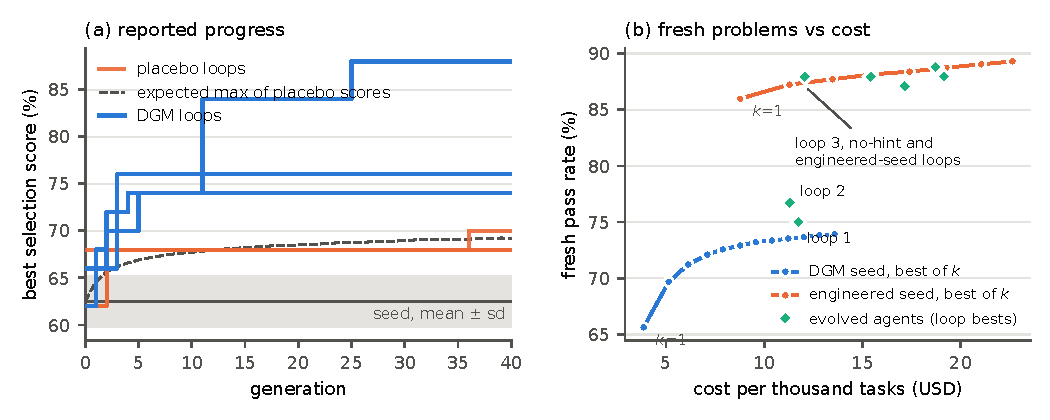
\includegraphics[width=\linewidth]{fig1.pdf}
\caption{First-round loops. (a) Best selection score by generation. Placebo loops (children are exact copies) rise to the expected
maximum of their own noisy scores (dashed); DGM loops rise above it. (b) Pass rate on $F_1$ against cost per task.
Lines: the unchanged seeds run $k$ times, submitting the first solution that passes the examples in the problem statement.
Diamonds: best agents of the loops.}\label{fig:main}
\end{figure}

\paragraph{Selection on noise.} The unchanged seed scores $\nseedDgmSmean\% \pm \nseedDgmSsd$ on $S$ over
$\nseedDgmSn$ evaluations (its own and those of placebo copies, which have identical code). The $\vhPlaceboN$ placebo
loops evaluate about 80 copies each on the full selection set and
report best scores of $\vhPlaceboMin$ to $\vhPlaceboMax\%$; the expected maximum of that many independent draws with the
seed's mean and spread is $\vhPlaceboPred\%$ (Figure~\ref{fig:main}a shows the three first-round placebo loops and the three first-round DGM loops). A loop's best
selection score therefore carries a noise term of about seven points, predictable from the rerun spread and the number of full evaluations. For the DGM
loops the selection gain exceeds the fresh gain in every loop, by about four points on average, but with each loop's
sampling error this is not significant (H2; \S\ref{sec:results2}).

\paragraph{Compute.} Evolved agents spend more per task than the seed. Rerunning the unchanged seed several times and
submitting the first solution that passes the examples in the problem statement (Table~\ref{tab:compute}) accounts for most
of the fresh gains of two of the three first-round loops at similar cost: their best agents differ from the
seed at matched cost by $\nvskLoopA$ [$\nvskLoopAlo$, $\nvskLoopAhi$] and $\nvskLoopB$ [$\nvskLoopBlo$, $\nvskLoopBhi$]
points on $F_1$. Resampling does not reproduce the third loop's gain even at twelve attempts, which still cost less
than that agent, probably because the seed fails the same problems on every attempt.

\paragraph{Repair.} The seed requests at most 4{,}096 output tokens. The task model's default reasoning often uses that
budget up on hard problems, and the agent then receives neither text nor a tool call and stops; $\nseedEmptyShare\%$ of
the seed's fresh runs end with no solution. Loop 3's best agent recovers from such empty turns by retrying with larger
budgets, nudges and fallback calls. Raising the seed's cap to 16{,}000 tokens and changing nothing else gains
$\vlvCapgain$ points [$\vlvCapgainlo$, $\vlvCapgainhi$] on all fresh problems in the final batch that re-evaluated every
loop agent together (Table~\ref{tab:loops}), where it trails loop 3's agent by $\vcapVsLoopFinAbs$ points [$\vcapVsLoopFinAbslo$,
$\vcapVsLoopFinAbshi$] at about a third of its cost per task; in the batch of the lineage ablation (\S\ref{sec:round2}) it trails by $\vcapvsloopthreeAbs$
[$\vcapvsloopthreeAbslo$, $\vcapvsloopthreeAbshi$]. The cap-only seed is an exploratory arm.

\paragraph{Other first-round results} (details in Appendix~\ref{app:round1}). Single edits proposed from the agent's
code alone gain about two points; single DGM steps gain 1.9 times as much when children that failed to compile count
as unchanged, and 2.7 times as much when those children are left out, mostly through the DGM's hand-written empty-patch prompt. Loops started from the engineered seed (a short harness that already avoids the empty-turn failure)
gain about two points on fresh problems (\nhFourCI). Under a bug in our first grader, most of the measured gain
of loops started from that harness was recovery from the bug; re-scoring the saved archives with the corrected grader
shows this without new agent runs. Under other task models, evolved agents gain most where the seed fails worst, and loop 3's agent costs
\ncostRatioRange{} times as much per task as the seed. These small first-round gains are measured against a seed reference that
pools runs from different hours (Appendix~\ref{app:round1}).

\begin{table}[t]\centering\small
\caption{The unchanged seed run $k$ times, submitting the first solution that passes the sample tests in the problem statement
($F_1$; averaged over orderings of the available runs). Cost in dollars per thousand tasks.}\label{tab:compute}
\begin{tabular}{lrrrrr}\toprule
 & $k=1$ & $k=2$ & $k=3$ & $k=6$ & $k=12$ \\ \midrule
DGM seed, pass rate & \natkDgmOne & \natkDgmTwo & \natkDgmThree & \natkDgmSix & \natkDgmTwelve \\
\quad cost & \natkDgmOneusd & \natkDgmTwousd & \natkDgmThreeusd & \natkDgmSixusd & \natkDgmTwelveusd \\ \bottomrule
\end{tabular}\end{table}

% Round-2 methods (pre-registered in PREREG_v2 before any round-2 run; deviations in Appendix~\ref{app:dev}).
\section{Baselines without self-improvement}\label{sec:round2}
The first round shows where the loops' gains come from. It does not show whether a loop was needed to find them. A
second pre-registration fixed four baselines (B1--B4 below: textbook moves, random diagnosis, one-shot redesign and a
lineage ablation; the placebo loops were registered in the first round), three generality checks,
and a test of published systems, before any of them ran.

\paragraph{Textbook moves (B1).} The engineered seed differs from the DGM seed in four files, and each difference is a
standard engineering move: E, a string-replace editor (view with line ranges, create, replace a unique string, insert);
B, a non-interactive shell with closed standard input, a per-command timeout and clipped output; L, a model loop that
allows 16{,}000 output tokens, answers every tool call in a response, re-prompts once after an output cut off by the
cap and stops after 40 turns; P, a workflow prompt that asks for sample tests, a brute-force cross-check and a timing
check. We build all 16 combinations by copying the chosen files into the DGM seed and evaluate each twice on all 232
fresh problems, interleaving agents problem by problem so that every agent sees the same hours.

\paragraph{Random diagnosis (B2).} Three loops run the DGM procedure unchanged except that each diagnosis is replaced by
one request drawn uniformly from a fixed list of 20 generic improvement requests (for example, ``Add a step that writes
a brute-force reference solution and compares it with the main solution on random small inputs''). The list was written
after the first round and before any second-round run; none of its requests mentions the output cap, but one asks the
agent to recover from responses that contain neither text nor a tool call, and two are close to it: one reruns the
agent when the solution file was not changed, and one logs the stop reason and usage of each response. This is search over textbook requests
instead of diagnoses.

\paragraph{One-shot redesign (B3).} A language model receives, once, the seed's code and the logs of five failed
selection-set runs of the seed (the material the DGM's diagnosis step sees) and returns the files it would change. It gets no evaluation
feedback. We draw five samples from Claude Opus~5.5 (pre-registered) and five from Claude Sonnet~5.5, the loops'
diagnosis model (added to separate the design from model strength). This is diagnosis without search.

\paragraph{Lineage ablation (B4).} For the best agent of each first-round DGM loop we rebuild the agent from the seed by
applying its lineage's patches in order, and build variants with one patch left out and with one patch alone. We
also revert the output cap in loop 3's best agent while keeping all its other code.

\paragraph{Generality.} Three more DGM loops and three more placebo loops on the same seed and tasks double the number of
loops per arm. Three loops replace the DGM's parent choice with HGM-style Thompson sampling: each archive member's
clade (the member and all its evaluated descendants) contributes its passed and failed selection runs to a Beta
posterior, and the parent is the member with the largest draw \citep{wang2026hgm}. Three DGM loops and one placebo loop
use gpt-oss-120b as task and self-editing model (20 generations). As an exploratory addition, two DGM loops and one
placebo loop use Claude Haiku~4.5, a model that rarely exhausts the seed's output cap, so that the cap fix is not
available to the search.

\paragraph{Analysis rules.} Gains and intervals are computed as in \S\ref{sec:setup}. These intervals hold the
realized loops fixed, so arm-level comparisons are also tested at the level of loops. Comparisons that pair agents from two batches (H6, H8 and the comparison of L with one retry in
\S\ref{sec:results2}) are reported as raw differences in the text and also seed-adjusted, with the batch times and seed
drifts, in Appendix~\ref{app:batches}. When a best candidate is chosen among several (15 combinations, five redesigns),
it is chosen on the first half of the fresh problems and compared on the second half, a rule fixed after the pre-registration
but before any result was summarized (Appendix~\ref{app:dev}, item 4); we also report the literal registered reading. The non-inferiority margin is
3 points. The final batch re-evaluates every loop's reported best agent, the seed, the cap-only seed and L
together on all fresh problems, twice.

\paragraph{Published systems.} For the DGM's SWE-bench run we rebuild the initial agent as it ran in 2025: the released
repository's history starts after the run, and two small differences from the run-time code (a later retry in the
model call and an example line in the editor) are inferred from the context lines of the archive's patches, after
which all six patches of the reported best agent's lineage apply without a rejected hunk. We compare the initial
agent, the reported best agent, the initial agent with textbook moves (the string-replace editor, a 16{,}000-token
output budget and five workflow steps in the prompt) and the same with up to three attempts selected by the
repository's regression tests, built from helper functions that the DGM's initial agent already contains. All four run
inside each task's container through the DGM's own harness, on SWE-bench Verified tasks outside the DGM's 200-task
evaluation set and on the DGM's 60 selection tasks, keeping only tasks whose reference patch passes under today's
environments. For ADAS we take the archived agent with the best validation score in each domain and compare it with
chain-of-thought self-consistency \citep{wang2023selfconsistency} given the same number of model calls, on ADAS's own
test sets, with Claude Haiku~5.5 replacing gpt-3.5. ADAS's search and evaluation code is imported unchanged; we
raise the output limit from 4{,}096 to 16{,}000 tokens for every agent, score a question 0 instead of aborting the run
when an agent raises an error, read every agent's JSON with the same tolerant parser, run 7 to 16 workers instead of
48, and send no sampling temperature, which the API no longer accepts.

\paragraph{Third round.} A third pre-registration, frozen after the second-round results and before any of its runs,
addressed three weaknesses of the first two rounds: the output limit that differs between the DGM's agents and the
textbook agent on SWE-bench, the random-diagnosis list, which contained a request aimed at empty responses, and the
failure logs that both the engineered seed and the one-shot redesigns had seen. It reruns the SWE-bench comparison at
equal output budget (\S\ref{sec:swe-equal}), makes one-shot redesigns without failure logs
(\S\ref{sec:redesign-logfree}) and repeats the random-diagnosis loops with a clean request list
(\S\ref{sec:random-clean}). Every primary contrast of this round is within one batch; Table~\ref{tab:hyp3} lists its
hypotheses (H11--H15) and verdicts.

\section{Results on competitive programming}\label{sec:results2}
\subsection{Textbook moves}
\begin{table}[t]\centering\small
\caption{Textbook moves added to the DGM seed (Haiku~5.5; all 232 fresh problems, two runs each, one interleaved batch).
E: string-replace editor; B: non-interactive shell; L: model loop with a 16{,}000-token budget; P: workflow prompt.
Gain over the seed in the same batch with 95\% intervals; cost in dollars per thousand tasks; share of runs that end
with no solution.}\label{tab:grid}
\begin{tabular}{lrrrr}\toprule
moves & $F$ (\%) & gain [95\% CI] & cost & no solution (\%) \\ \midrule
\csname @@input\endcsname tab_grid.tex
\bottomrule\end{tabular}\end{table}
Every combination that contains the model-loop move L gains between $\vgridWithLmin$ and $\vgridWithLmax$ points over
the seed, and every combination without it between $\vgridNoLmin$ and $\vgridNoLmax$ (Table~\ref{tab:grid}). L bundles
four changes (a 16{,}000-token budget, an answer to every tool call, one re-prompt after a truncated output, and a
40-turn limit); alone it gains $\vgridLgain$ points. The editor and the shell change nothing measurable on their own, and the workflow prompt alone costs
$\vgridPgainAbs$ points: its longer reasoning runs into the seed's 4{,}096-token cap more often.

\paragraph{The registered test (H6).} The second pre-registration asks whether the best textbook combination comes
within three points of the best first-round loop agent, the one from loop 3. The best of the 15 combinations is chosen
on $F_1$ and compared on $F_2$ (\S\ref{sec:round2}); we also named two single candidates to report on all of $F$, all
four moves and L. Loop 3's agent was re-evaluated in another batch, so these contrasts cross batches. We report raw
contrasts here and seed-adjusted ones in Appendix~\ref{app:batches}. All contrasts in this paragraph are the candidate minus loop 3's agent, in points.

The combination chosen on $F_1$ (\vHsixWinner) is $\vHsixFtwoAbs$ points [$\vHsixFtwoAbslo$, $\vHsixFtwoAbshi$] behind
on $F_2$, so H6 is not supported. Over the \vlcN{} combinations that contain L, the contrasts on $F_2$ range from
$\vlcFtwoMin$ to $\vlcFtwoMax$, and the chosen one happens to be the lowest. On all of $F$, all four moves are
$\vpsEBLPRawAbs$ points [$\vpsEBLPRawAbslo$, $\vpsEBLPRawAbshi$] behind and L is $\vpsLRawAbs$ [$\vpsLRawAbslo$,
$\vpsLRawAbshi$] behind. Of the \vlcN{} L combinations, \vlcMiss{} miss the margin and \vlcSig{} are significantly behind.
The literal registered reading chooses the best combination on all of $F$ (\vhsixLitBest) and scores it on the same
problems, which favours it; its contrast, $\vhsixLit$ [$\vhsixLitlo$, $\vhsixLithi$], is within the margin on raw scores
but not after seed adjustment. Every combination is cheaper per task than loop 3's agent, at most
$\vgridMaxCostShare\%$ of its cost; L alone costs $\vgridLCostShare\%$ as much, and all four moves
cost $\vgridEBLPCostShare\%$. Measured from the seed, the textbook moves thus close about nine tenths of the distance to the
best loop agent and remain one to five points behind it: on all fresh problems the contrasts of the L combinations range
from $\vlcFMax$ to $\vlcFMin$, and on $F_2$ the chosen combination is at $\vHsixFtwo$.

\paragraph{All loops against one move (exploratory).} The final batch measured every loop's reported best agent, the
seed, the cap-only seed and L together, two runs per problem (Table~\ref{tab:loops}). There L gains $\vlvLgain$ points
[$\vlvLgainlo$, $\vlvLgainhi$] over the seed. No loop agent is significantly better than L and $\vlvWorse$ of $\vlvN$
are significantly worse; the best, loop 3's agent, is $\vlvBest$ points [$\vlvBestlo$, $\vlvBesthi$] ahead, so
non-inferiority of L within three points is not shown in this batch either. In the third-round batch, loop 3's agent is
$\rcLoopThreeLAbs$ points [$\rcLoopThreeLAbslo$, $\rcLoopThreeLAbshi$] ahead of L, a significant gap
(\S\ref{sec:random-clean}). Section~\ref{sec:round1} reports how far the cap-only seed trails loop 3's agent in the final
and ablation batches. The proxy caps every request at 16{,}000 output tokens, so loop 3's agent never receives more output
than L; what it adds is more attempts after an empty turn. With one more attempt when its first solution fails the
sample tests in the problem statement (the rule of the compute-matched baseline above), L reaches $\vLtwoAcc\%$ at
\$$\vLtwoUsd$ per thousand tasks, while loop 3's agent reaches $\vLthreeAcc\%$ at \$$\vLthreeUsd$, a contrast of
$\vltwoRaw$ points [$\vltwoRawlo$, $\vltwoRawhi$]. This comparison pairs L's runs from the grid batch with loop 3's agent
from the ablation batch (Appendix~\ref{app:batches}); it was specified after the H6 result and before it was computed.

\subsection{One-shot redesigns}
\begin{table}[t]\centering\small
\caption{One-shot redesigns of the DGM seed by a language model (Haiku~5.5 task model; fresh problems, two runs each).
Each redesign saw the seed's code and five failure logs once. Cap: the output cap the redesign set. Opus redesigns are
registered; Sonnet redesigns are exploratory.}\label{tab:redesign}
\begin{tabular}{lrrrr}\toprule
agent & cap & $F$ (\%) & gain [95\% CI] & cost \\ \midrule
\csname @@input\endcsname tab_redesign.tex
\bottomrule\end{tabular}\end{table}
Four of the five Opus redesigns and three of the five Sonnet redesigns raise the output cap to 8{,}192 tokens and gain
18 to 22 points; the three that keep 4{,}096 change the pass rate by $-1$ to $+8$ points (Table~\ref{tab:redesign}). For
the registered H8 we take contrasts as redesign minus loop, again across batches (Appendix~\ref{app:batches}). The
contrast of the average Opus redesign with the average loop best is $\vHeightOpusmean$ [$\vHeightOpusmeanlo$,
$\vHeightOpusmeanhi$], so this part is supported. The best of five, chosen on $F_1$, is $\vHeightOpusbestAbs$ points
[$\vHeightOpusbestAbslo$, $\vHeightOpusbestAbshi$] behind loop 3's agent on $F_2$, so that part is not. The best Opus
redesign on all of $F$ is $\vheightLitOpusRawAbs$ points [$\vheightLitOpusRawAbslo$, $\vheightLitOpusRawAbshi$] behind.

\paragraph{Without failure logs.}\label{sec:redesign-logfree} In the third round, five further samples from Claude Opus~5.5 received the redesign
prompt without the five failure logs: the agent summary, the seed's code and the same task paragraph. Four of the five
raise the output cap to 8{,}192 tokens, as four of five did with the logs; the fifth keeps 4{,}096 but continues after a
truncated response and reruns the agent when no solution was written. In one batch with the seed, which scores $\lfSeedF\%$, the
log-free redesigns gain $\lfGainMin$ to $\lfGainMax$ points, on average $\lfMeanFree$ [$\lfMeanFreelo$, $\lfMeanFreehi$],
compared with $\lfMeanBased$ [$\lfMeanBasedlo$, $\lfMeanBasedhi$] for the redesigns made from failure logs; the difference is
$\lfDiff$ points [$\lfDifflo$, $\lfDiffhi$], so the registered non-inferiority test passes. An exploratory comparison shows that the
averages agree for different reasons. Among the redesigns that raise the cap, those made without logs gain $\lfRaiseDiffAbs$
points [$\lfRaiseDiffAbslo$, $\lfRaiseDiffAbshi$] less than those made from logs. Of the two that keep 4{,}096, the
log-free one gains $\lfKeepFree$ points and the log-based one gains $\lfKeepBased$. Claude Opus~5.5 thus finds the fix from the code
alone when asked for a one-shot redesign, so the failure logs are not needed to find it. In the first round, none of the
\nladConeatt{} diagnoses that Claude Sonnet~5.5 made from the agent's code alone mentions the output cap, stop reasons or
empty responses (Appendix~\ref{app:round1}).


\subsection{Search without diagnosis, another search rule, more loops}
\begin{table}[t]\centering\small
\caption{Reported best agents of all Haiku~5.5 loops, re-evaluated together with the seed in one batch (all 232 fresh
problems, two runs each). $S$: the selection score for which the loop reported the agent. Inflation: selection gain
over the seed's pooled selection score ($\nseedDgmSmean\%$ over $\nseedDgmSn$ evaluations) minus fresh gain. Cost in dollars per thousand tasks. The first-round DGM loops and the second-round
arms (more DGM loops, random diagnosis, HGM-style) are registered; the loops without hint prompts are exploratory. The
last rows are references measured in the same batch.}\label{tab:loops}
\begin{tabular}{llrrrr}\toprule
loop type & loop & $S$ & fresh gain [95\% CI] & inflation & cost \\ \midrule
\csname @@input\endcsname tab_loops.tex
\bottomrule\end{tabular}\end{table}
The random-diagnosis loops draw every request from the fixed list of \S\ref{sec:round2}; because one request targets
empty responses, they search over textbook requests rather than without any diagnosis. In the final batch they gain $\vhRandom$ points [$\vhRandomlo$, $\vhRandomhi$] on average,
whereas the first-round DGM loops gain $\vhDgmTwo$ [$\vhDgmTwolo$, $\vhDgmTwohi$]. The registered non-inferiority test
(H7) fails: the difference is $\vhRandomMinusDgm$ [$\vhRandomMinusDgmlo$, $\vhRandomMinusDgmhi$]. Against all six DGM
loops it is $\vhRandomMinusDgmAll$ [$\vhRandomMinusDgmAlllo$, $\vhRandomMinusDgmAllhi$]. HGM-style parent selection gains
$\vhHgm$ [$\vhHgmlo$, $\vhHgmhi$], which is $\vhHgmMinusDgmAllAbs$ [$\vhHgmMinusDgmAllAbslo$, $\vhHgmMinusDgmAllAbshi$]
points more than the six DGM loops (Table~\ref{tab:loops}). These intervals resample problems (\S\ref{sec:round2}). Compared at the
level of loops (three or six per arm), none of the arm differences is significant (Welch tests: HGM-style vs DGM
$p=\vllHgmP$, random vs first-round DGM $p=\vllRandomThreeP$, random vs all DGM $p=\vllRandomSixP$). Four of the 14 loops
reach the level of the single move L: loop 3, both loops without hint prompts and one HGM-style loop; one of the six DGM
loops does.

For each DGM loop the selection gain exceeds the fresh gain, by $\vhtwoMinInfl$ to $\vhtwoMaxInfl$ points. With each
loop's own sampling error (tasks resampled, as registered for H2) every interval includes zero, and over the six loops
the hierarchical estimate is $\vhtwoMean$ points [$\vhtwoLo$, $\vhtwoHi$]. The placebo loops' best selection scores
are given in \S\ref{sec:round1}.


\paragraph{With a clean request list.}\label{sec:random-clean}
Five loops ran the DGM procedure with every diagnosis replaced by a request drawn from a clean list, and three DGM loops
ran at the same time. The clean list is the second-round list with the three failure-related requests described in
\S\ref{sec:round2} replaced by three generic ones. The one aimed at empty responses also
asked the agent to answer every tool call, which is part of move L. In the third-round batch, which also re-evaluated the earlier loops' agents and where the seed scores $\rcSeedF\%$, the five clean
random-diagnosis loops
gain $\rcClean$ points [$\rcCleanlo$, $\rcCleanhi$] on average, with individual loops from $\rcCleanMin$ to
$\rcCleanMax$. All nine DGM loops gain $\rcDgmAll$ [$\rcDgmAlllo$, $\rcDgmAllhi$], and the three that ran at the same
time $\rcDgmNew$ [$\rcDgmNewlo$, $\rcDgmNewhi$]. The registered non-inferiority test fails: the clean loops trail the DGM loops
by $\rcHfourteenAbs$ points [$\rcHfourteenAbslo$, $\rcHfourteenAbshi$], and at the level of loops the difference is
significant (Welch test, $p=\rcHfourteenP$). The registered secondary contrast, against the three same-time DGM loops,
is $\rcCleanNew$ [$\rcCleanNewlo$, $\rcCleanNewhi$] ($p=\rcCleanNewP$).

The remaining contrasts in this batch are exploratory. The random-diagnosis loops of the second round gain $\rcRandOld$
[$\rcRandOldlo$, $\rcRandOldhi$]. That is
$\rcCleanOldAbs$ points [$\rcCleanOldAbslo$, $\rcCleanOldAbshi$] more than the clean loops ($p=\rcCleanOldP$) and level
with all nine DGM loops ($\rcRandAll$ [$\rcRandAlllo$, $\rcRandAllhi$]). The same-time DGM loops reproduce the earlier
ones within $\rcNewOldAbs$ points. Search over generic requests therefore gains much less when no request points at the
failure, and the DGM's diagnosis, which reads the failure logs, does better. The single model-loop move L gains $\rcL$
[$\rcLlo$, $\rcLhi$] in this batch, more than the average DGM loop but $\rcLoopThreeLAbs$ points [$\rcLoopThreeLAbslo$,
$\rcLoopThreeLAbshi$] less than the agent of loop 3.


\subsection{What the lineages contain}
The loops' edits depend on each other. Removing one edit from a lineage and re-applying the rest leaves rejected hunks
for all but \vlinThreeClean{} of loop 3's \vlinThreeN{} edits (\vlinTwoClean{} of \vlinTwoN{} for loop 2, \vlinOneClean{}
of \vlinOneN{} for loop 1), so the registered test of whether two edits carry most of the gain (H9) cannot be run.
Removing loop 3's last edit, the only leave-one-out variant that applies cleanly, costs $\vlasteditAbs$ points
[$\vlasteditAbslo$, $\vlasteditAbshi$]. In an exploratory variant, setting the output cap of loop 3's agent back to 4{,}096 tokens while keeping
its other code costs only $\vsemcapdropAbs$ points [$\vsemcapdropAbslo$, $\vsemcapdropAbshi$], probably because the
agent also retries empty turns with nudges and fallback calls.

\section{Published systems}\label{sec:published}
\subsection{The DGM's SWE-bench agents}
\begin{table}[t]\centering\small
\caption{The DGM's released SWE-bench agents and the initial agent with textbook moves, run through the DGM's own
harness with Claude Sonnet~4.5 on SWE-bench Verified tasks whose reference patch passes today: fresh tasks outside the
DGM's evaluation set, and the DGM's selection tasks. One run per task. Early: runs, of all 293, in which the agent
process ended before the harness recorded a patch; they count as unresolved.}\label{tab:swe}
\setlength{\tabcolsep}{4pt}
\begin{tabular}{lrrrr}\toprule
agent & fresh & DGM selection & \$/run & early \\ \midrule
DGM initial agent & \vsweInitFreshN/\vsweInitFreshOf\ (\vsweInitFresh\%) & \vsweInitSelN/\vsweInitSelOf & \vsweInitUsd & \vsweInitEarly \\
DGM reported best agent & \vsweBestFreshN/\vsweBestFreshOf\ (\vsweBestFresh\%) & \vsweBestSelN/\vsweBestSelOf & \vsweBestUsd & \vsweBestEarly \\
initial + textbook moves & \vsweMovesFreshN/\vsweMovesFreshOf\ (\vsweMovesFresh\%) & \vsweMovesSelN/\vsweMovesSelOf & \vsweMovesUsd & \vsweMovesEarly \\
\quad + regression-test retries & \vsweRetryFreshN/\vsweRetryFreshOf\ (\vsweRetryFresh\%) & \vsweRetrySelN/\vsweRetrySelOf & \vsweRetryUsd & \vsweRetryEarly \\ \bottomrule
\end{tabular}\end{table}
The DGM reports that its search took the initial agent from 20\% to 50\% on its 200 SWE-bench tasks with Claude~3.5
Sonnet, which is no longer served. We ran all four agents with Claude Sonnet~4.5 on Verified tasks outside the DGM's
200-task evaluation set (Table~\ref{tab:swe}); Sonnet~4.5 is newer than the model the DGM used. As run in the DGM's harness, the reported best agent resolves $\vsweBestMinusInitAbs$ points
[$\vsweBestMinusInitAbslo$, $\vsweBestMinusInitAbshi$] fewer fresh tasks than the initial agent it came from, and the
initial agent with three textbook moves (defined in \S\ref{sec:round2}) resolves $\vsweMovesMinusBestAbs$ points [$\vsweMovesMinusBestAbslo$, $\vsweMovesMinusBestAbshi$] more
than the best agent, at about a quarter of its cost per task. The textbook moves alone add $\vsweMovesMinusInitAbs$ points
[$\vsweMovesMinusInitAbslo$, $\vsweMovesMinusInitAbshi$] to the initial agent at the same cost. On the DGM's own selection
tasks the textbook agent leads the best agent by $\vsweMovesMinusBestSelAbs$ points [$\vsweMovesMinusBestSelAbslo$,
$\vsweMovesMinusBestSelAbshi$].

Most of the best agent's deficit relative to its initial agent comes from runs that end early. In \vsweBestEarly{} of
its \vsweBestRuns{} runs the agent process ended before the harness recorded a patch, and the DGM's harness then discards the
run, as it does for every agent. We could not determine the cause for this model; the exit codes, a scan of the saved
logs and two pilots are described in Appendix~\ref{app:swe}. The best agent's design (up to three attempts, each checked
with the repository's regression tests, plus summarization of long conversations) produces long sessions: its median
run took \vsweBestMedMin{} minutes, compared with \vsweMovesMedMin{} for the textbook agent. Among the runs that finished, the best
agent resolves the largest share of fresh tasks ($\vsweBestFinFresh\%$; the textbook
agent resolves $\vsweMovesFinFresh\%$), but this comparison conditions on finishing and favours agents that end early on hard tasks.

In an exploratory sensitivity analysis, we graded the patch that each early-ended run left in the repository, as if
the harness had kept it. This does not show what a completed run would have produced. Of the best agent's
\vsweBestEarly{} early-ended runs, \vsensBestPatched{} had a patch, and \vsensBestPatchedResolved{} of those resolve their
task. With these patches kept, the best agent resolves $\vsensBestFresh\%$ of fresh tasks. That is $\vsensBestMinusInit$
points [$\vsensBestMinusInitlo$, $\vsensBestMinusInithi$] relative to the initial agent, and the textbook agent
($\vsensMovesFresh\%$) still leads it by $\vsensMovesMinusBestAbs$ points [$\vsensMovesMinusBestAbslo$,
$\vsensMovesMinusBestAbshi$]. On the DGM's selection tasks, with patches kept, the textbook agent's lead shrinks to
$\vsensMovesMinusBestSelAbs$ points [$\vsensMovesMinusBestSelAbslo$, $\vsensMovesMinusBestSelAbshi$], and the best agent
is $\vsensBestMinusInitSel$ [$\vsensBestMinusInitSello$, $\vsensBestMinusInitSelhi$] relative to its initial agent. Under
this newer model, then, neither reading of the fresh tasks shows a significant gain for the released best agent over
the initial agent it came from, and the textbook agent remains ahead of it. The advantage the DGM reported (from 20\% to 50\%) does not carry over.

\paragraph{At equal output budget.}\label{sec:swe-equal} The DGM's initial and reported best agents allow at
most 4{,}096 output tokens in each tool-calling request, and the textbook agent allows 16{,}000. We raised this limit of
both DGM agents to 16{,}000 and changed nothing else (other model calls, such as the best agent's summaries of its history, keep 4{,}096 in all three agents), and in the third round ran the
three agents in one batch on $\wN$ of the fresh tasks, drawn at random, with half the earlier parallelism. The textbook
agent resolves $\wMovesRate\%$ of the tasks at \$\wMovesUsd{} per task run, the initial agent resolves $\wInitRate\%$
at \$\wInitUsd{}, and the best agent resolves $\wBestRate\%$ at \$\wBestUsd{}. The textbook agent leads the best agent by
$\wMovesBestAbs$ points [$\wMovesBestAbslo$, $\wMovesBestAbshi$] (McNemar $p=\wMovesBestP$), so the registered
non-inferiority test passes and the lead is significant, and the best agent is $\wBestInitAbs$ points
[$\wBestInitAbslo$, $\wBestInitAbshi$] below its own initial agent ($p=\wBestInitP$). The initial agent is
$\wMovesInitAbs$ points [$\wMovesInitAbslo$, $\wMovesInitAbshi$] below the textbook agent, which is not significant
($p=\wMovesInitP$).

The best agent still ends \wBestEarly{} of its \wN{} runs early, compared with \wInitEarly{} for the initial agent and
\wMovesEarly{} for the textbook agent, although the machine was far less loaded than in the earlier batch and memory
pressure does not explain the endings (Appendix~\ref{app:dev}, items 13 and 14). With the patches of early-ended runs
kept, the textbook agent still leads the best agent by $\wsMovesBestAbs$ points [$\wsMovesBestAbslo$,
$\wsMovesBestAbshi$], and the best agent is $\wsBestInitAbs$ points [$\wsBestInitAbslo$, $\wsBestInitAbshi$] below its
initial agent, which is not significant ($p=\wsBestInitP$).


\paragraph{Harness findings.} The DGM's harness runs the task's evaluation script inside the agent's container before
the agent starts, to install the environment. That script applies the hidden tests, runs them and restores only the test
files it modified. Afterwards a pytest cache directory remained in all 106 pytest-based tasks we ran (of 293; the django and sympy
tasks use their own test runners); in the
three we inspected, its \texttt{lastfailed} file named the failing hidden tests: in two it listed exactly the test that
the reference patch must make pass, and in the third those 4 tests among 142.
Test files that the hidden patch adds also stay in the repository (8 of 300 fresh and 7 of the DGM's 200 tasks). To our knowledge this has not been reported; the nearest known case is agents reading
future commits from the repository's history \citep{swebench2025issue465}. None of the DGM's released chats reads the
cache, so its reported numbers do not appear to use it, but a self-modifying agent could learn to. All our runs remove
this residue after setup. Separately, 59 of the 352 tasks we built no longer pass with their reference patch under
today's package versions and were excluded for every agent.

\subsection{ADAS}
\begin{table}[t]\centering\small
\caption{ADAS's best-by-validation discovered agents (found with gpt-3.5) against chain-of-thought self-consistency
with a matched number of samples (one extra aggregation call on DROP), both run with Claude Haiku~5.5 on ADAS's test
sets. Calls per question in parentheses. Last column: the gain over CoT-SC that ADAS's archive reports with gpt-3.5 (for
DROP computed from archive medians that lie above their own reported intervals).}\label{tab:adas}
\footnotesize\setlength{\tabcolsep}{3pt}
\begin{tabular}{lrrrrrr}\toprule
domain & ADAS agent & CoT-SC & CoT & agent $-$ CoT-SC [95\% CI] & agent $-$ CoT & archive gain \\ \midrule
\csname @@input\endcsname tab_adas.tex
\bottomrule\end{tabular}\end{table}
Run with a current model, ADAS's discovered agents lose to self-consistency with matched calls on MGSM and DROP, tie on
MMLU and win on GPQA (Table~\ref{tab:adas}); a single chain-of-thought call matches or beats them on three of four
domains with a quarter to a tenth of the calls. On DROP the discovered agent gives longer answers, which ADAS's own F1 metric penalizes: on the items where it
scores below CoT-SC, its answer is longer in \vdropWorseLonger{} of \vdropWorse{} (median \vdropLenAgent{} characters,
compared with \vdropLenCot{}). The agents with the best test score in the archive behave the same way (on MGSM it is the same agent). This agrees with
\citet{jwalapuram2026illusion}, who find automatically designed multi-agent systems behind CoT-SC with current models.

\section{Related work}\label{sec:related}
\paragraph{Self-improving agents and automated agent design.} The DGM \citep{zhang2026dgm} and the Huxley-G\"odel
Machine \citep{wang2026hgm} let coding agents rewrite their own code and select variants on benchmark scores; ADAS
\citep{hu2025adas}, AFlow \citep{zhang2025aflow} and agentic harness engineering \citep{lin2026ahe} search over agent
designs or workflows; the G\"odel Agent \citep{yin2025godel}, SICA \citep{robeyns2025sica}, STOP \citep{zelikman2023stop}
and Hyperagents \citep{zhang2026hyperagents} make the improver itself editable. Some recent systems report gains that
transfer to held-out benchmarks and models \citep{srikanth2026aide2,lin2026ahe}.

\paragraph{How such gains should be measured.} Selection on a small benchmark inflates reported scores
\citep{hu2026winners,cawley2010overfitting}. Harness evolution often fails to beat test-time scaling at
matched budgets \citep{wang2026rethinking}, and LLM-driven program evolution loses most of its advantage over
independent sampling at matched token budgets \citep{oved2026tokens}; much of harness evolution's gain splits into
overfitting and extra inference \citep{ding2026hda}. A pre-registered study finds that prompt and parser search on small models mostly repairs
a capped-thinking mismatch that a setting change also repairs \citep{xu2026harnessrepair}, close to our cap result. In
test generation, once the oracle is audited, equal-budget resampling beats evolution and a placebo feedback loop comes
within about two points of real feedback \citep{liang2026testgen}; placebo-controlled retries at matched budgets also
match execution feedback on small code models \citep{verma2026tryagain}, and an evolving harness repairs process
failures rather than content failures \citep{tian2026ceiling}. Edits in the DGM's logs repair their target failure no more often than other failures
\citep{he2026failurefeedback}; re-executing the DGM's SWE-bench evaluations leaves its decisions unchanged
\citep{ding2026reexecuting}; and few published self-improvement studies compare improvers at matched budgets from identical starting points
\citep{chen2026auditing}. Meta-agents rarely match human-engineered baselines \citep{lu2026metaagent}, while a one-shot
rewrite did not explain the gains of one open-ended optimizer \citep{xue2026rethinking}, in contrast to our one-shot
redesigns. Automatically designed multi-agent systems lose to CoT-SC with current models
\citep{jwalapuram2026illusion}. For DGM-style self-modifying loops, our study adds exact-copy placebo loops, textbook-move and one-shot-redesign
baselines, search over a list of textbook requests, and a re-run of the DGM's own released agents on fresh tasks.

\paragraph{Baselines and evaluation hygiene.} Random search matched neural architecture search under equal budgets
\citep{li2019random,yang2020nas}, and seed variance changed conclusions in deep reinforcement learning
\citep{henderson2018deep}; agent evaluations should also control cost \citep{kapoor2024agents}, and repeated sampling or
self-consistency are strong references \citep{brown2024monkeys,wang2023selfconsistency}. SWE-bench
\citep{jimenez2024swebench,openai2024swebenchverified} has known leaks and weak tests
\citep{swebench2025issue465,ludwig2026shortcutting,aleithan2024swebenchplus,wang2025solved}, agentic benchmarks often have
setup and reward flaws \citep{zhu2025abc}, and agents exploit visible checks when they can
\citep{gabor2025evilgenie,zhong2026impossiblebench}.

\section{Discussion}\label{sec:discussion}
\begin{table}[t]\centering\footnotesize
\caption{Pre-registered hypotheses of the first two rounds (H1--H5, H6--H10), the estimate with its 95\% interval and
the verdict. (a) marks amendments made before the results; (p) marks readings or tests chosen after the results.
Contrasts are candidate minus comparator. Contrasts across batches are raw; seed-adjusted values are in Table~\ref{tab:batches}.}\label{tab:hyp}
\setlength{\tabcolsep}{3pt}
\begin{tabular}{>{\raggedright\arraybackslash}p{0.30\linewidth}>{\raggedright\arraybackslash}p{0.47\linewidth}>{\raggedright\arraybackslash}p{0.16\linewidth}}\toprule
hypothesis (as registered) & estimate & verdict \\ \midrule
H1 placebo loops show a positive selection gain of predictable size & first-round best scores inside leave-one-out
predictive intervals; six loops $\vhPlaceboMin$--$\vhPlaceboMax\%$ vs $\vhPlaceboPred\%$ predicted & supported \\
H2 DGM loops' selection gain exceeds their fresh gain; fresh gain positive & per-loop excess (tasks resampled)
$\vhtwoMinInfl$ to $\vhtwoMaxInfl$ points, every interval includes 0; six loops (hierarchical) $\vhtwoMean$
[$\vhtwoLo$, $\vhtwoHi$]; fresh gains all positive & not supported \\
H3 best log-free edit reaches $\geq 0.8\times$ the loops' fresh gain & (a) on $F_1$: ratio $\vhThreeRatio$ & not
supported \\
H4 from the engineered seed, fresh gains of all arms within $\pm 3$ points, selection gains $> 0$ & DGM loops:
\nhFourCI{} on $F$ (p: 90\% two one-sided tests) and $+\ngainStrongB$ [$\ngainStrongBlo$, $\ngainStrongBhi$] on $F_1$;
single-edit arms ($F_1$): $\nladSCone$ [$\nladSConelo$, $\nladSConehi$] and $\nladSCtwo$ [$\nladSCtwolo$,
$\nladSCtwohi$]; selection gains of the loops $+\nSgainStrongA$ and $+\nSgainStrongB$ & not supported (equivalence not
shown) \\
H5 evolved-agent gains shrink or vanish under Haiku~4.5 and Sonnet~4.6 & (a) on $F_1$, loops 1 and 3 (loop 2's agent
not run); change of gain, loop 3's agent: $\vhfiveKThree$ [$\vhfiveKThreelo$, $\vhfiveKThreehi$], $\vhfiveSThree$
[$\vhfiveSThreelo$, $\vhfiveSThreehi$]; loop 1's: $\vhfiveKOne$ [$\vhfiveKOnelo$, $\vhfiveKOnehi$], $\vhfiveSOne$
[$\vhfiveSOnelo$, $\vhfiveSOnehi$] & supported only for loop 3 under Sonnet~4.6 \\ \midrule
H6 best textbook combination $\geq$ best first-round loop agent $-3$ (and cheaper) & (a) chosen on $F_1$
(\vHsixWinner), on $F_2$: $\vHsixFtwo$ [$\vHsixFtwolo$, $\vHsixFtwohi$]; literal, best on all of $F$ (\vhsixLitBest; chosen and scored on the same problems):
$\vhsixLit$ [$\vhsixLitlo$, $\vhsixLithi$], seed-adjusted $\vhsixLitAdj$ [$\vhsixLitAdjlo$, $\vhsixLitAdjhi$]; (a)
pre-specified single candidates on all of $F$: all four moves $\vpsEBLPRaw$ [$\vpsEBLPRawlo$, $\vpsEBLPRawhi$], L
$\vpsLRaw$ [$\vpsLRawlo$, $\vpsLRawhi$]; all cheaper & not supported; literal reading supported on raw scores, not
after seed adjustment \\
H7 random-diagnosis loops $\geq$ first-round DGM loops $-3$ (mean fresh gain) & $\vhRandomMinusDgm$ [$\vhRandomMinusDgmlo$,
$\vhRandomMinusDgmhi$]; (p) vs six DGM loops $\vhRandomMinusDgmAll$ [$\vhRandomMinusDgmAlllo$, $\vhRandomMinusDgmAllhi$]
& not supported \\
H8 best of five one-shot redesigns $\geq$ best loop agent $-3$; mean redesign $\geq$ mean loop best $-3$ & (a) best on
$F_2$: $\vHeightOpusbest$ [$\vHeightOpusbestlo$, $\vHeightOpusbesthi$]; literal, best on all of $F$:
$\vheightLitOpusRaw$ [$\vheightLitOpusRawlo$, $\vheightLitOpusRawhi$]; mean: $\vHeightOpusmean$ [$\vHeightOpusmeanlo$,
$\vHeightOpusmeanhi$] & best: not supported; mean: supported \\
H9 two edits carry $\geq 80\%$ of a loop's fresh gain & loop 1 has exactly two edits; for loop 2 half and for loop 3
all but one of the leave-one-out variants do not apply & not testable (loops 2, 3) \\
H10 seed $+$ textbook moves ($+$ retry) $\geq$ published best $-3$ on fresh tasks & (a; pilot results known) DGM
SWE-bench with Sonnet~4.5, moves: $\vsweMovesMinusBest$ [$\vsweMovesMinusBestlo$, $\vsweMovesMinusBesthi$] as run,
$\vsensMovesMinusBest$ [$\vsensMovesMinusBestlo$, $\vsensMovesMinusBesthi$] with early-ended patches kept; moves and
retries: $\vsweRetryMinusBest$ [$\vsweRetryMinusBestlo$, $\vsweRetryMinusBesthi$] and $\vsensRetryMinusBest$
[$\vsensRetryMinusBestlo$, $\vsensRetryMinusBesthi$]; ADAS (CoT-SC vs agent): holds on MGSM, DROP, MMLU, fails on
GPQA; HGM and DGM Polyglot not run & (a) supported for DGM SWE-bench; 3 of 4 for ADAS \\ \bottomrule
\end{tabular}\end{table}

\begin{table}[t]\centering\footnotesize
\caption{Pre-registered hypotheses of the third round (H11--H15), the estimate with its 95\% interval and the
verdict. Every contrast is within one batch.}\label{tab:hyp3}
\setlength{\tabcolsep}{3pt}
\begin{tabular}{>{\raggedright\arraybackslash}p{0.30\linewidth}>{\raggedright\arraybackslash}p{0.47\linewidth}>{\raggedright\arraybackslash}p{0.16\linewidth}}\toprule
hypothesis (as registered) & estimate & verdict \\ \midrule
H11 at equal output budget, seed $+$ textbook moves $\geq$ DGM best agent $-3$ (SWE-bench) & as run
$\wMovesBest$ [$\wMovesBestlo$, $\wMovesBesthi$]; early-ended patches kept $\wsMovesBest$ [$\wsMovesBestlo$,
$\wsMovesBesthi$] & supported (also superior) \\
H12 at equal output budget, DGM best agent vs its initial agent (expected: no significant gain) & as run $\wBestInit$
[$\wBestInitlo$, $\wBestInithi$]; patches kept $\wsBestInit$ [$\wsBestInitlo$, $\wsBestInithi$] & no gain; worse as
run \\
H13 (descriptive) textbook agent vs initial agent with the raised limit & $\wMovesInit$ [$\wMovesInitlo$,
$\wMovesInithi$] & -- \\
H14 clean random-diagnosis loops $\geq$ all DGM loops $-3$ (mean fresh gain) & $\rcHfourteen$ [$\rcHfourteenlo$,
$\rcHfourteenhi$] & \rcHfourteenVerdict \\
H15 log-free redesigns: $\geq 4$ of 5 raise the cap; mean gain $\geq$ log-based $-3$ & \lfRaised{} of 5;
$\lfDiff$ [$\lfDifflo$, $\lfDiffhi$] & supported \\ \bottomrule
\end{tabular}\end{table}

Tables~\ref{tab:hyp} and~\ref{tab:hyp3} list the registered hypotheses and their outcomes, and the findings in the introduction
summarize them together with the exploratory comparisons. Read together, they show that the loops mostly
found standard engineering, which a one-shot redesign also reaches at a lower cost per task whether or not it sees
failure logs; they do not show that loops find nothing.

Two readings follow. The first concerns what search contributes. In most of our settings, a baseline that uses no
search (textbook moves, or a single redesign from the same failure logs) reached the level of the loops' best agents,
or came within a few points of it, at lower cost. The exceptions run both ways: on gpt-oss-120b an agent found by a loop
on another model gained more than our textbook set did, in a comparison across batches, and ADAS's discovered agent wins on GPQA.
Diagnosis also carries information: once the request list contains nothing aimed at the empty-turn failure,
random-diagnosis loops gain much less than DGM loops (\S\ref{sec:random-clean}). The loops' costs are
many evaluations and inflated selection scores (\S\ref{sec:round1}). The second reading concerns transfer to a
new task model. A harness is tuned to the model it was built for, whether by a loop or directly: the engineered seed
loses to the DGM seed under gpt-oss-120b, and it is ahead of loop 3's agent under Haiku~4.5 and Sonnet~4.6, about
level under Sonnet~5.5, and behind it under gpt-oss-120b and Gemini~2.5 Flash (Appendix~\ref{app:round1}). Published
self-improvement results should therefore be re-measured when the task model changes.

\paragraph{Recommendations.} Claims of self-improvement should report (i) gains on tasks that no selection step saw,
(ii) a placebo loop or its order-statistics prediction, (iii) the seed resampled at the agent's cost, (iv) the seed
with textbook moves and a one-shot redesign from the same failure logs, measured in the same batch as the loop's agent
(our own registered tests did not fully meet this), and (v) the released agent re-run with a newer model. Harnesses
should keep hidden tests out of the agent's container, keep the agent's work when its process ends early, and check that
each task's reference patch still passes.

\paragraph{Limitations.} Loops were run on one task family with one to nine loops per arm, and the confidence intervals
over problems hold the realized loops fixed. At the level of loops, differences between loop types are significant only
for the clean random-diagnosis loops of the third round (\S\ref{sec:random-clean}). The SWE-bench and other-model evaluations use one run per task, and budget and time limits censor several
agents under other models (Appendix~\ref{app:cens}). Claude~3.5 Sonnet, the DGM's original model, is no longer served,
so we cannot separate the effect of the model change from a failure to replicate. We could not determine what ends the
best agent's runs early under Claude Sonnet~4.5; machine load and memory do not explain it (\S\ref{sec:swe-equal}). The SWE-bench batch at equal output budget used \wN{} tasks. HGM's released agent and the DGM's Polyglot agents were not run. The proxy caps output at 16{,}000 tokens for
every arm. The engineered seed, the source of the textbook moves, was written while pilot runs that included \vnpN{}
of the fresh problems took place, and their logs showed the DGM seed's empty responses, so the textbook moves are not
independent of what failure logs show; without those problems the main numbers barely change (Appendix~\ref{app:pilot}).
The request list of the second-round random-diagnosis loops was drafted after the first round had exposed the
empty-turn failure, and three of its requests aim at or near it (\S\ref{sec:round2}); the third round repeats the test
without them (\S\ref{sec:random-clean}). Several
comparisons were added after earlier results (Appendix~\ref{app:dev}, items 3 and 15); those of item 3 were specified
before they were computed, and those of item 15 after they were computed. Under Haiku~4.5 most runs of the DGM seed end with its agent process killed by a signal, which the engineered
seed avoids (Appendix~\ref{app:othermodels}). Heavy load on the shared machine affected part of one exploratory batch
and the last generations of three loops, and the second-round SWE-bench run used an oversubscribed machine
(Appendix~\ref{app:dev}).


\clearpage
\section*{Code and data availability}
Code, the three pre-registrations, the change log and per-task results are available at
\url{https://doi.org/10.5281/zenodo.23719813}; the same files are on GitHub at
\url{https://github.com/tejasvi/self-improving-agents-textbook-baselines} (tag v3).

\section*{Acknowledgements}
Generative AI tools were used to write code, run analyses and draft text; the author directed the work and takes full responsibility for its content.

\bibliographystyle{plainnat}
\bibliography{refs_v2}

\clearpage
\appendix
\section{Changes after pre-registration}\label{app:dev}
The three pre-registrations and the full log of changes (DEVIATIONS.md) are in the release; this is a summary. The
pre-registrations call the engineered seed the strong or hand-written seed (\texttt{seed\_strong} in the released files).
\begin{enumerate}\setlength{\itemsep}{1pt}\renewcommand{\labelenumi}{(\arabic{enumi})}
\item The first launch was aborted because proxy restarts dropped model calls.
\item The first grader shadowed the built-in \texttt{pow}; the campaign was relaunched with a corrected grader, and five
old-grader loops were kept for the grader analysis.
\item Exploratory comparisons added after earlier results: the loops without hint prompts, the cap-only seed, the
compute-matched resampling baseline and its follow-up for L, the reversal of the output cap in loop 3's agent, the
Sonnet redesigns, the loops
and textbook moves with Claude Haiku~4.5, the textbook moves, one-shot redesigns and resampled seed under gpt-oss-120b,
the first-round transfer runs under Claude Sonnet~5.5, Gemini~2.5 Flash and gpt-oss-120b, the ADAS agents with the best
test score, and the SWE-bench sensitivity analysis. Each was specified before it was computed.
\item The rule that chooses a best candidate on $F_1$ and compares it on $F_2$ (H6, H8) was fixed after the second
pre-registration, while the grid batch was running (about three quarters done) and before any result was summarized
(we had only glanced at the first 100 runs for crashes);
the literal reading is reported as well.
\item H6, H8 and the L comparison pair agents from different batches. The pre-registration's same-batch seeds ``to
control drift'' and the pre-results rule that comparisons use same-batch references point to seed-adjusted contrasts,
while the pre-results rule that names loop 3's agent re-evaluated ``in the same period'' as the comparator fits raw
ones; none of
them says explicitly how such contrasts are formed. The analysis code, written before the comparator's batch finished,
computed raw contrasts, and seed-adjusted contrasts were added after the raw contrasts had been computed. Verdicts are given under both; they differ
only for the literal reading of H6, which fails under the seed-adjusted contrast.
\item H2: the round-2 summary over six loops is given with the registered per-loop task bootstrap and a hierarchical
bootstrap; an earlier analysis used a bootstrap over loop means only.
\item The random-diagnosis list of the second round was written after the first round had identified the empty-turn
failure (\S\ref{sec:round2}); the third round replaced the requests aimed at it (\S\ref{sec:random-clean}).
\item Pilot overlap with the fresh problems: Appendix~\ref{app:pilot}.
\item Proxy spending caps were raised during the runs; evolved agents get one fresh run per problem in the first round;
the improver swap used 12 diagnoses instead of 16.
\item H9 could not be run as registered for loops 2 and 3, because half (loop 2) or all but one (loop 3) of the
leave-one-out variants do not apply. H3 and H5 are computed on $F_1$ instead of $F$, because the single edits and the
transfer runs were evaluated on $F_1$ only; H5 covers loops 1 and 3, because loop 2's agent was not run under the other
models (to limit cost). H4 is reported for every arm started from the engineered seed.
\item In the registered SWE-bench test of the DGM, Claude Haiku~4.5 was replaced by Claude Sonnet~4.5 after a pilot in which most runs of both DGM
agents ended early; the outcomes of a 15-task pilot with Claude Sonnet~4.5 (Appendix~\ref{app:swe}), including resolve
rates, were known when the model and protocol of the full run were fixed; the
registered Claude Haiku~5.5 runs were not made; the third textbook move is a workflow prompt
rather than a loop change; the retry arm costs less than the best agent instead of the same; tasks whose reference
patch fails today were excluded for all agents; hidden-test residue is removed from the agent's container after setup.
\item The registered test of HGM's released agent was not run, because the agent supports only OpenAI's Responses API,
and the registered test of the DGM on its Polyglot benchmark was not run.
\item Part of one exploratory batch and the selection runs of three loops near their end ran during heavy load on the
shared machine (re-grading that batch's saved solutions changed 5 of 1{,}624 outcomes); later batches ran on a separate
machine. During the second-round SWE-bench run the machine's CPU was oversubscribed (per-run mean load up to \vloadMax{} on 64
cores). Load was sampled every minute over the whole run in \vloadFullPct\% of runs and over part of it in
\vloadPartPct\%, and interpolated from checks every 30 minutes for the rest, including \vloadMovesApprox{} of the
textbook agent's 293 runs. By load tertile (low, middle, high), the
early-ending rates were: initial agent \vearlyInitLo, \vearlyInitMid{} and \vearlyInitHi\%; best agent \vearlyBestLo,
\vearlyBestMid{} and \vearlyBestHi\%; textbook agent \vearlyMovesLo, \vearlyMovesMid{} and \vearlyMovesHi\%; retry
variant \vearlyRetryLo, \vearlyRetryMid{} and \vearlyRetryHi\%. The resolve rate of the textbook agent fell from
\vresMovesLo\% to \vresMovesHi\%, which works against it. The tertiles are formed per
agent and are confounded with run order, so these figures do not rule out an effect of load. In the third round the
one-minute load average stayed below \wLoadMax{} (in the second round it reached \wvLoadMax), and the best agent still
ended \wBestEarly{} of \wN{} runs early, compared with \wvBestEarly{} on the same tasks in the second round (\S\ref{sec:swe-equal}).
\item Third round: the loops ran with eight task workers each instead of twelve (parallelism only) on a spot machine
that was preempted three times during the runs, twice during the loops and once during the third-round batch. Each time the
jobs resumed from their saved state, and an unfinished child or run was redone. The spending cap of that machine was
raised by \$40 before the third-round batch, and its third-round spend was \$331.66, against the \$330 registered. The
SWE-bench machine reached the internet only through address translation, and the requirement files that the swebench
code reads from GitHub were served from a local copy of the same files. The third-round SWE-bench run used eight task containers per agent,
half the earlier parallelism. Comparisons with the second round's SWE-bench runs on the same tasks are exploratory, because they cross
batches. In the third-round SWE-bench run, the early endings of the best agent were \wBestEarlySig{} on a signal and \wBestEarlyOne{} with exit code 1,
all those of the other two agents were on a signal, and \wBestEarlyBoth{} of the best agent's tasks end early in both rounds.
The kernel logged one out-of-memory kill; none of the \wOomInProg{} runs then in progress ended early within ten minutes of
it, and \wOomEarlyLater{} of them ended early at least \wOomGapMin{} minutes later. With the patches of early-ended runs
kept, the three agents resolve \wMovesKept\%, \wInitKept\% and \wBestKept\% (textbook, initial, best), and the initial
agent is \wsMovesInitAbs{} points below the textbook agent ($p=\wsMovesInitP$). In an exploratory comparison of the same
tasks between the second-round batch and this one, the rate of the best agent changes by $\wxBest$ points [$\wxBestlo$,
$\wxBesthi$] and that of the initial agent by $\wxInit$ [$\wxInitlo$, $\wxInithi$], while the textbook agent reproduces
its earlier rate within $\wxMovesAbs$ points; the two batches differ in the output limit, the parallelism and the machine
load.
\item Third round: exploratory analyses first computed during internal review and then added: the second-round
random-diagnosis loops against the DGM loops in the third-round batch, loop 3's agent against L in that batch, the redesigns
that raise the cap with and without logs, the runs in progress at the out-of-memory kill, and the second-round early
endings on the same 65 tasks.
\end{enumerate}

\section{Contrasts across batches}\label{app:batches}
H6, H8 and the comparison of L with one retry pair agents from different batches. Loop 3's agent was re-evaluated in the
ablation batch (\vbtAbl{} UTC), which started together with the grid batch of the 16 combinations (\vbtGrid{} UTC) and
was about a quarter done when the grid ended; the redesign batch ran within the ablation batch's hours (\vbtRed{} UTC).
Relative to the seed in the grid batch, the seed in the ablation batch scores $\vsvAblGridF$ points [$\vsvAblGridFlo$,
$\vsvAblGridFhi$] on all of $F$. Relative to the seed in the redesign batch, it scores $\vsvAblRedFtwo$
[$\vsvAblRedFtwolo$, $\vsvAblRedFtwohi$] on $F_2$ and $\vsvAblRedF$ [$\vsvAblRedFlo$, $\vsvAblRedFhi$] on all of $F$, so
raw contrasts are less favourable to the redesigns than seed-adjusted ones by these amounts. A seed-adjusted contrast is
(candidate minus its batch's seed) minus (comparator minus its batch's seed), paired by problem; item 5 of
Appendix~\ref{app:dev} explains why both are given. Table~\ref{tab:batches} lists both. The verdicts agree except for the
literal reading of H6, which passes on raw scores and fails after seed adjustment.
\begin{table}[h]\centering\small
\caption{Contrasts across batches, raw and seed-adjusted (candidate minus comparator, in points, with 95\%
intervals).}\label{tab:batches}
\begin{tabular}{p{0.46\linewidth}lll}\toprule
contrast & problems & raw & seed-adjusted \\ \midrule
H6: combination chosen on $F_1$ (\vHsixWinner) vs loop 3's agent & $F_2$ & $\vHsixFtwo$ [$\vHsixFtwolo$, $\vHsixFtwohi$] & $\vbaHsix$ [$\vbaHsixlo$, $\vbaHsixhi$] \\
H6, literal: best combination on $F$ (\vhsixLitBest) vs loop 3's agent & $F$ & $\vhsixLit$ [$\vhsixLitlo$, $\vhsixLithi$] & $\vhsixLitAdj$ [$\vhsixLitAdjlo$, $\vhsixLitAdjhi$] \\
all four moves vs loop 3's agent & $F$ & $\vpsEBLPRaw$ [$\vpsEBLPRawlo$, $\vpsEBLPRawhi$] & $\vpsEBLPAdj$ [$\vpsEBLPAdjlo$, $\vpsEBLPAdjhi$] \\
L vs loop 3's agent & $F$ & $\vpsLRaw$ [$\vpsLRawlo$, $\vpsLRawhi$] & $\vpsLAdj$ [$\vpsLAdjlo$, $\vpsLAdjhi$] \\
H8: average Opus redesign vs average loop best & $F$ & $\vHeightOpusmean$ [$\vHeightOpusmeanlo$, $\vHeightOpusmeanhi$] & $\vbaOpusMean$ [$\vbaOpusMeanlo$, $\vbaOpusMeanhi$] \\
H8: best of five Opus redesigns (chosen on $F_1$) vs loop 3's agent & $F_2$ & $\vHeightOpusbest$ [$\vHeightOpusbestlo$, $\vHeightOpusbesthi$] & $\vbaOpusBest$ [$\vbaOpusBestlo$, $\vbaOpusBesthi$] \\
H8, literal: best Opus redesign on $F$ vs loop 3's agent & $F$ & $\vheightLitOpusRaw$ [$\vheightLitOpusRawlo$, $\vheightLitOpusRawhi$] & $\vheightLitOpusAdj$ [$\vheightLitOpusAdjlo$, $\vheightLitOpusAdjhi$] \\
L with one retry vs loop 3's agent & $F$ & $\vltwoRaw$ [$\vltwoRawlo$, $\vltwoRawhi$] & $\vltwoAdj$ [$\vltwoAdjlo$, $\vltwoAdjhi$] \\
\bottomrule\end{tabular}\end{table}

\section{Pilot overlap}\label{app:pilot}
The engineered seed, and with it the textbook moves E, B, L and P, was written while two short pilot runs of the DGM
seed took place, and their logs were read as it was written. The second pilot covered 80 problems, \vnpN{} of which
are in $F$ (and 7 in the selection set); the first used a subset of them. Of the second pilot's \vpilotRuns{} runs,
\vpilotNoSol{} ended without a solution, \vpilotEmptyResp{} of them on an empty response, the failure that L repairs.
L is therefore a repair informed by failure logs, like a one-shot redesign, rather than a move chosen without them. Without those problems, L gains $\vnpLgain$ points [$\vnpLgainlo$,
$\vnpLgainhi$] in the final batch, no loop agent is significantly better than L and $\vnpWorse$ are significantly worse
(best: $\vnpLoopThreeVsL$ [$\vnpLoopThreeVsLlo$, $\vnpLoopThreeVsLhi$]), and the H6 contrast on $F_2$ is $\vnpHsix$
[$\vnpHsixlo$, $\vnpHsixhi$].

\section{Other task models}\label{app:othermodels}
These comparisons are exploratory.
\paragraph{Claude Haiku~4.5.} This model rarely reaches the seed's cap ($\vkMaxTok\%$ of the seed's responses stop at
it, among runs with logs), but another failure takes its place: in $\vsigKSeed\%$ of the seed's runs the agent process is killed by a signal
before it finishes (\vsigKSeedTr\% in the first-round transfer runs; \vsigHSeed\% under Haiku~5.5). The chat logs
of these runs are empty, because the seed writes its log on exit; in the SWE-bench pilot with the same model, such
endings came from cleanup commands that the agent itself ran (Appendix~\ref{app:swe}). A batch of single textbook moves under this
model, in which the seed scores $\vkgNoneF\%$, separates the causes. The non-interactive shell B removes the signal endings
entirely (\vkgBSig\% of runs, compared with \vkgNoneSig\% for the seed) and gains $\vkgBgain$ points [$\vkgBgainlo$,
$\vkgBgainhi$]; the editor, the model loop and the workflow prompt alone show no gain ($\vkgEgain$, $\vkgLgain$ and
$\vkgPgain$ points), and their runs still end on a signal in about three quarters of cases. All four moves together gain
$\vkgEBLPgain$ points [$\vkgEBLPgainlo$, $\vkgEBLPgainhi$], $\vkgBMinusEBLPAbs$ more than the shell alone. Of the two
loops, one found nothing ($\vkOnegain$ [$\vkOnegainlo$, $\vkOnegainhi$] in the final batch; \vsigKOne\% of its runs end
on a signal). The other gained $\vkTwogain$ points [$\vkTwogainlo$, $\vkTwogainhi$] at \$$\vkTwoUsd$ per thousand tasks
with four edits that rebuild parts of the engineered seed's workflow (repeated attempts with the previous failure in
context, a brute-force reference with random stress tests, timing on a maximum-size input, and a rule never to stop with
a known time-out); \vsigKTwo\% of its runs end on a signal, and others reach the budget or the time limit
(Appendix~\ref{app:cens}). The seed resampled eight times, at a lower cost than that agent, is $\vkTwoMatchedAbs$ points
[$\vkTwoMatchedAbslo$, $\vkTwoMatchedAbshi$] below it on $F_1$, so its gain is not a compute effect alone.
The engineered seed, which combines the shell fix with the workflow, is $\vkStrongMinusTwo$ points
[$\vkStrongMinusTwolo$, $\vkStrongMinusTwohi$] ahead of it at a lower cost in the final batch, where the seed scores $\vkSeedF\%$. The Haiku~4.5
placebo loop's best selection score (34\%) lies between those of the two loops (28\% and 40\%).

\paragraph{gpt-oss-120b.} This model is slow: depending on the agent, \vtoOssMin{} to \vtoOssMax\% of its runs reach
the 600\,s limit, and the solution present at that point is graded (Appendix~\ref{app:cens}). In the final batch for
this model the DGM seed solves $\voSeedF\%$ of the fresh problems; the engineered seed scores $\voStronggainAbs$ points
below it. One of three loops gained $\voOnegain$ points [$\voOnegainlo$, $\voOnegainhi$], with a workflow prompt and the
rule to write the solution file at once and never end a turn without it; its best agent costs about three times as much
per task as the seed, and the seed resampled \vossSkK{} times at a similar cost reaches $\vossSkAcc\%$ on $F_1$, and the
contrast of the loop agent with it there is $\vossLoopMinusSk$ points [$\vossLoopMinusSklo$, $\vossLoopMinusSkhi$]. A
second loop's reported agent has a fresh gain of $\voThreegain$ [$\voThreegainlo$, $\voThreegainhi$] and reaches the 600\,s limit in
\vtoOssThree\% of its runs, and the third never got a child through the
full selection set; neither did any of the placebo loop's 40 copies. In a separate batch
of single textbook moves, in which the seed scores $\vogNoneF\%$, the moves as written for Haiku~5.5 do not transfer: the editor alone
scores $\vogEgainAbs$ points below the seed, the move chosen on $F_1$ (\vogWinner) gains $\vogLgain$ [$\vogLgainlo$,
$\vogLgainhi$], and the loop's agent, measured in the same batch, is ahead of that move by $\vogWinnerFtwoAbs$
[$\vogWinnerFtwoAbslo$, $\vogWinnerFtwoAbshi$] on $F_2$. Loop 3's agent from the first round, evolved with Haiku~5.5,
gained $\ntrOssthree$ points [$\ntrOssthreelo$, $\ntrOssthreehi$] on $F_1$ in the first-round transfer runs
(Appendix~\ref{app:round1}), more than any textbook move gains in the batch above; the two numbers come from different
batches. This is consistent with the retries after empty turns that the loop found transferring where our textbook set
does not, but we did not ablate them under this model.
In a third batch we evaluated five one-shot redesigns made from five failure logs of this model. The best of five,
chosen on $F_1$, beats the loop's agent on $F_2$ by $\vorBestVsLoop$ points [$\vorBestVsLooplo$, $\vorBestVsLoophi$]; the average of the five
trails it by $\vorMeanVsLoopAbs$ [$\vorMeanVsLoopAbslo$, $\vorMeanVsLoopAbshi$], because one redesign was broken and
solved nothing. Choosing the best of five used 116 evaluated problems, more than the loops' 50-problem selection set.


\section{Time and budget limits}\label{app:cens}
This appendix gives the shares of runs that end on a signal, reach the wall-clock limit, or spend at least 99\% of the
per-run budget, for the batches in which any of these is common. In the final batch under Claude Haiku~4.5 (\$1
budget), the DGM seed ends on a signal in \vsigKSeed\% of runs (\vsigKSeedTr\% in the transfer runs) and the
engineered seed in \vsigKStrong\%; the engineered seed reaches the budget in \vbudKStrong\%. Loop 1's agent ends on a
signal in \vsigKOne\% of runs and reaches the time limit in \vtoKOne\%. Loop 2's agent ends on a signal in
\vsigKTwo\%, reaches the time limit in \vtoKTwo\% and the budget in \vbudKTwo\%. In the first-round transfer runs,
loop 3's agent reaches the \$1 budget in \vbudTrKThreeN{} of 116 runs under Claude Haiku~4.5 and in \vbudTrSThreeN{}
under Claude Sonnet~4.6, and the DGM seed ends on a signal in \vsigSSeed\% of its Sonnet~4.6 runs. Under gpt-oss-120b
no run ends on a signal, and the share of runs that reach the 600\,s limit ranges from 47 to 100\% across agents in the
final batch, from 14 to 60\% in the textbook-move batch and from 28 to 94\% in the redesign batch. In the Haiku~5.5
final batch at most 1\% of runs end on a signal; time-outs reach 22\% for one loop agent and are under 10\% for every
other agent. Pass rates under these limits are censored from above.

\section{First-round details}\label{app:round1}
\begin{table}[h]\centering\small
\caption{Single edits of the DGM seed and log-free chains (the diagnosis sees only the agent's code, no task log). Fresh gain on $F_1$ averaged over evaluated members, the same
average counting children that failed to compile as unchanged, and the member with the best selection score.}\label{tab:ladder}
\footnotesize\setlength{\tabcolsep}{3pt}
\begin{tabular}{lrrrrrr}\toprule
diagnosis given to the editing step & tried & failed & evaluated & mean gain [95\% CI] & with failures & best-by-$S$ \\ \midrule
agent code only (no task data) & \nladConeatt & \nladConefail & \nladConen & $\nladCone$ [$\nladConelo$, $\nladConehi$] & $\nladConeitt$ & $\nladConebest$ \\
task log, no hint prompts & \nladCthreeatt & \nladCthreefail & \nladCthreen & $\nladCthree$ [$\nladCthreelo$, $\nladCthreehi$] & $\nladCthreeitt$ & $\nladCthreebest$ \\
DGM diagnosis (task log and hint prompts) & \nladCtwoatt & \nladCtwofail & \nladCtwon & $\nladCtwo$ [$\nladCtwolo$, $\nladCtwohi$] & $\nladCtwoitt$ & $\nladCtwobest$ \\
log-free chain 1 (steps) & \nladDoneatt & \nladDonefail & \nladDonen & $\nladDone$ [$\nladDonelo$, $\nladDonehi$] & $\nladDoneitt$ & $\nladDonebest$ \\
log-free chain 2 (steps) & \nladDtwoatt & \nladDtwofail & \nladDtwon & $\nladDtwo$ [$\nladDtwolo$, $\nladDtwohi$] & $\nladDtwoitt$ & $\nladDtwobest$ \\ \bottomrule
\end{tabular}\end{table}
\paragraph{Single edits.} A diagnosis model that sees only the agent's code proposes plausible generic changes; none
of its \nladConeatt{} diagnoses mentions the output cap, stop reasons or empty responses. Implemented by the seed, the
changes gain about two points on average (Table~\ref{tab:ladder}), about the same as edits from a
task log without the DGM's hint prompts. Single DGM steps gain two to three times as much (counting children that
failed to compile as unchanged, or not); the children that came from the empty-patch prompt carry that gain, and all children from the stochasticity prompt failed to produce a working
edit. Log-free chains mostly broke the agent. These single-edit gains, and the two-point gains of loops started from the
engineered seed, are measured against a pooled seed reference whose morning runs scored about 2.5 points higher than
its evening runs, so they depend on the reference to within about that much.

\paragraph{Grader quirk.} Our first grader prepended \texttt{from math import *} to every solution, which replaces the
built-in \texttt{pow} and breaks \texttt{pow(a, b, m)}. Loops from the engineered seed proposed tools that run a
solution under several import preludes. Re-scoring the saved archives with the corrected grader shows that most of
their measured gain (\nquirkStrongMeasText{} on the selection set) was recovery from the bug (\nquirkStrongCorrText{}
corrected); the two graders rank the archives with Spearman $\rho=\nQArho$ and $\nQBrho$.

\paragraph{Improver swap.} The same twelve DGM diagnoses of the seed were implemented on a fresh copy of the seed by
the seed agent and by loop 3's best agent. \nswapText{} Among the evolved agent's finished edits, \nswapLinesText{}. A
better coding agent does not yield more working agents from the same instructions.

\begin{table}[h]\centering\small
\caption{First-round agents under other task models ($F_1$, one run per problem, \$1 budget, \$0.25 for gpt-oss-120b).
Gains are paired against the DGM seed under the same model; budget and time limits censor some agents
(Appendix~\ref{app:cens}).}\label{tab:transfer}
\begin{tabular}{lrrrr}\toprule
task model & DGM seed & engineered seed & loop-3 best: gain & loop-1 best: gain \\ \midrule
Claude Haiku~4.5 & \ntrHfourseed & \ntrHfourstrong & $\ntrHfourthree$ [$\ntrHfourthreelo$, $\ntrHfourthreehi$] & $\ntrHfourone$ [$\ntrHfouronelo$, $\ntrHfouronehi$] \\
Claude Sonnet~4.6 & \ntrSfourseed & \ntrSfourstrong & $\ntrSfourthree$ [$\ntrSfourthreelo$, $\ntrSfourthreehi$] & $\ntrSfourone$ [$\ntrSfouronelo$, $\ntrSfouronehi$] \\
Claude Sonnet~5.5 & \ntrSfiveseed & \ntrSfivestrong & $\ntrSfivethree$ [$\ntrSfivethreelo$, $\ntrSfivethreehi$] & $\ntrSfiveone$ [$\ntrSfiveonelo$, $\ntrSfiveonehi$] \\
Gemini~2.5 Flash & \ntrGemseed & \ntrGemstrong & $\ntrGemthree$ [$\ntrGemthreelo$, $\ntrGemthreehi$] & $\ntrGemone$ [$\ntrGemonelo$, $\ntrGemonehi$] \\
gpt-oss-120b & \ntrOssseed & \ntrOssstrong & $\ntrOssthree$ [$\ntrOssthreelo$, $\ntrOssthreehi$] & $\ntrOssone$ [$\ntrOssonelo$, $\ntrOssonehi$] \\ \bottomrule
\end{tabular}\end{table}

\section{SWE-bench details}\label{app:swe}
\paragraph{Rebuilding the agents.} The released DGM repository starts after the SWE-bench run. Its initial agent
differs from the run-time agent in two places that the archive's patch contexts reveal: a later retry around the model
call and an example line in the editor. With both restored, the six patches of the reported best agent's lineage
apply in order without a rejected hunk. The textbook agents start from the restored initial agent; the retry variant
uses helper functions the initial agent already contains (regression-test discovery, test runs and a report score).

\paragraph{Protocol.} All four agents run through the DGM's harness with one change (each task gets its own proxy token
and the proxy address), on 246 fresh tasks (SWE-bench Verified minus the DGM's 200, minus tasks whose environment does
not build or whose reference patch fails today) and 47 of the DGM's 60 selection tasks, one run per task, \$10 per run,
16 tasks in parallel per agent, all four agents at once in the same task order. A pilot with Claude Haiku~4.5 was
stopped because most runs of both DGM agents ended early; Claude Sonnet~4.5 was used instead. A 15-task pilot with
it showed 7 of the best agent's 14 runs and 3 of the initial agent's 15 runs ending early; the full run kept the same
protocol. Grading follows the DGM's
own report script; evaluations that timed out were re-graded alone. One task (scikit-learn-14710) timed out in
evaluation for both textbook agents even when re-graded alone and counts as unresolved; in the sensitivity analysis one
patch of the best agent (psf\_\_requests-1142) got no report and counts as unresolved.

\paragraph{Early endings.} Of the best agent's \vsweBestEarly{} early endings in the second-round run, \vsweBestEarlySig{} came on
a signal (exit codes 137 and 143) and \vsweBestEarlyOne{} with exit code 1. Of the saved logs of these runs, \vsweKillEmpty{} are
empty; \vsweKillLogs{} of the other \vsweKillNonEmpty{} contain a command that ends processes (\texttt{pkill}, \texttt{killall}
or \texttt{kill -9}), and \vsweKillNone{} contain no such command. In the pilot with Claude Haiku~4.5 we traced such endings to
cleanup commands issued through the agent's own shell. Median run times were \vsweInitMedMin{} minutes for the initial
agent and \vsweRetryMedMin{} for the retry variant; among the runs that finished, the retry variant resolves
$\vsweRetryFinFresh\%$ and the initial agent $\vsweInitFinFresh\%$ of the fresh tasks.

\section{Costs}\label{app:cost}
Model spend was about \$4{,}600 for the competitive-programming study (all three rounds) and the ADAS test together,
and about \$3{,}700 for the SWE-bench tests; machine time was small by comparison. These totals cover the model calls of the
experiments only.

\end{document}
